
%% bare_conf.tex
%% V1.3
%% 2007/01/11
%% by Michael Shell
%% See:
%% http://www.michaelshell.org/
%% for current contact information.
%%
%% This is a skeleton file demonstrating the use of IEEEtran.cls
%% (requires IEEEtran.cls version 1.7 or later) with an IEEE conference paper.
%%
%% Support sites:
%% http://www.michaelshell.org/tex/ieeetran/
%% http://www.ctan.org/tex-archive/macros/latex/contrib/IEEEtran/
%% and
%% http://www.ieee.org/

%%*************************************************************************
%% Legal Notice:
%% This code is offered as-is without any warranty either expressed or
%% implied; without even the implied warranty of MERCHANTABILITY or
%% FITNESS FOR A PARTICULAR PURPOSE! 
%% User assumes all risk.
%% In no event shall IEEE or any contributor to this code be liable for
%% any damages or losses, including, but not limited to, incidental,
%% consequential, or any other damages, resulting from the use or misuse
%% of any information contained here.
%%
%% All comments are the opinions of their respective authors and are not
%% necessarily endorsed by the IEEE.
%%
%% This work is distributed under the LaTeX Project Public License (LPPL)
%% ( http://www.latex-project.org/ ) version 1.3, and may be freely used,
%% distributed and modified. A copy of the LPPL, version 1.3, is included
%% in the base LaTeX documentation of all distributions of LaTeX released
%% 2003/12/01 or later.
%% Retain all contribution notices and credits.
%% ** Modified files should be clearly indicated as such, including  **
%% ** renaming them and changing author support contact information. **
%%
%% File list of work: IEEEtran.cls, IEEEtran_HOWTO.pdf, bare_adv.tex,
%%                    bare_conf.tex, bare_jrnl.tex, bare_jrnl_compsoc.tex
%%*************************************************************************

% *** Authors should verify (and, if needed, correct) their LaTeX system  ***
% *** with the testflow diagnostic prior to trusting their LaTeX platform ***
% *** with production work. IEEE's font choices can trigger bugs that do  ***
% *** not appear when using other class files.                            ***
% The testflow support page is at:
% http://www.michaelshell.org/tex/testflow/



% Note that the a4paper option is mainly intended so that authors in
% countries using A4 can easily print to A4 and see how their papers will
% look in print - the typesetting of the document will not typically be
% affected with changes in paper size (but the bottom and side margins will).
% Use the testflow package mentioned above to verify correct handling of
% both paper sizes by the user's LaTeX system.
%
% Also note that the "draftcls" or "draftclsnofoot", not "draft", option
% should be used if it is desired that the figures are to be displayed in
% draft mode.
%
\documentclass[10pt, conference, compsocconf]{IEEEtran}
% Add the compsocconf option for Computer Society conferences.
%
% If IEEEtran.cls has not been installed into the LaTeX system files,
% manually specify the path to it like:
% \documentclass[conference]{../sty/IEEEtran}





% Some very useful LaTeX packages include:
% (uncomment the ones you want to load)


% *** MISC UTILITY PACKAGES ***
%
%\usepackage{ifpdf}
% Heiko Oberdiek's ifpdf.sty is very useful if you need conditional
% compilation based on whether the output is pdf or dvi.
% usage:
% \ifpdf
%   % pdf code
% \else
%   % dvi code
% \fi
% The latest version of ifpdf.sty can be obtained from:
% http://www.ctan.org/tex-archive/macros/latex/contrib/oberdiek/
% Also, note that IEEEtran.cls V1.7 and later provides a builtin
% \ifCLASSINFOpdf conditional that works the same way.
% When switching from latex to pdflatex and vice-versa, the compiler may
% have to be run twice to clear warning/error messages.



\pdfminorversion=4
\pdfimageresolution=300


% *** CITATION PACKAGES ***
%
\usepackage{cite}
% cite.sty was written by Donald Arseneau
% V1.6 and later of IEEEtran pre-defines the format of the cite.sty package
% \cite{} output to follow that of IEEE. Loading the cite package will
% result in citation numbers being automatically sorted and properly
% "compressed/ranged". e.g., [1], [9], [2], [7], [5], [6] without using
% cite.sty will become [1], [2], [5]--[7], [9] using cite.sty. cite.sty's
% \cite will automatically add leading space, if needed. Use cite.sty's
% noadjust option (cite.sty V3.8 and later) if you want to turn this off.
% cite.sty is already installed on most LaTeX systems. Be sure and use
% version 4.0 (2003-05-27) and later if using hyperref.sty. cite.sty does
% not currently provide for hyperlinked citations.
% The latest version can be obtained at:
% http://www.ctan.org/tex-archive/macros/latex/contrib/cite/
% The documentation is contained in the cite.sty file itself.

\usepackage{listings}

% *** GRAPHICS RELATED PACKAGES ***
%
\ifCLASSINFOpdf
   \usepackage[pdftex]{graphicx}
  % declare the path(s) where your graphic files are
  \graphicspath{{../pdf/}{../jpeg/}}
  % and their extensions so you won't have to specify these with
  % every instance of \includegraphics
   \DeclareGraphicsExtensions{.pdf,.jpeg,.png}
\else
  % or other class option (dvipsone, dvipdf, if not using dvips). graphicx
  % will default to the driver specified in the system graphics.cfg if no
  % driver is specified.
  % \usepackage[dvips]{graphicx}
  % declare the path(s) where your graphic files are
  % \graphicspath{{../eps/}}
  % and their extensions so you won't have to specify these with
  % every instance of \includegraphics
   \DeclareGraphicsExtensions{.eps}
\fi
% graphicx was written by David Carlisle and Sebastian Rahtz. It is
% required if you want graphics, photos, etc. graphicx.sty is already
% installed on most LaTeX systems. The latest version and documentation can
% be obtained at: 
% http://www.ctan.org/tex-archive/macros/latex/required/graphics/
% Another good source of documentation is "Using Imported Graphics in
% LaTeX2e" by Keith Reckdahl which can be found as epslatex.ps or
% epslatex.pdf at: http://www.ctan.org/tex-archive/info/
%
% latex, and pdflatex in dvi mode, support graphics in encapsulated
% postscript (.eps) format. pdflatex in pdf mode supports graphics
% in .pdf, .jpeg, .png and .mps (metapost) formats. Users should ensure
% that all non-photo figures use a vector format (.eps, .pdf, .mps) and
% not a bitmapped formats (.jpeg, .png). IEEE frowns on bitmapped formats
% which can result in "jaggedy"/blurry rendering of lines and letters as
% well as large increases in file sizes.
%
% You can find documentation about the pdfTeX application at:
% http://www.tug.org/applications/pdftex





% *** MATH PACKAGES ***
%
\usepackage[cmex10]{amsmath}
% A popular package from the American Mathematical Society that provides
% many useful and powerful commands for dealing with mathematics. If using
% it, be sure to load this package with the cmex10 option to ensure that
% only type 1 fonts will utilized at all point sizes. Without this option,
% it is possible that some math symbols, particularly those within
% footnotes, will be rendered in bitmap form which will result in a
% document that can not be IEEE Xplore compliant!
%
% Also, note that the amsmath package sets \interdisplaylinepenalty to 10000
% thus preventing page breaks from occurring within multiline equations. Use:
%\interdisplaylinepenalty=2500
% after loading amsmath to restore such page breaks as IEEEtran.cls normally
% does. amsmath.sty is already installed on most LaTeX systems. The latest
% version and documentation can be obtained at:
% http://www.ctan.org/tex-archive/macros/latex/required/amslatex/math/





% *** SPECIALIZED LIST PACKAGES ***
%
%\usepackage{algorithmic}
% algorithmic.sty was written by Peter Williams and Rogerio Brito.
% This package provides an algorithmic environment fo describing algorithms.
% You can use the algorithmic environment in-text or within a figure
% environment to provide for a floating algorithm. Do NOT use the algorithm
% floating environment provided by algorithm.sty (by the same authors) or
% algorithm2e.sty (by Christophe Fiorio) as IEEE does not use dedicated
% algorithm float types and packages that provide these will not provide
% correct IEEE style captions. The latest version and documentation of
% algorithmic.sty can be obtained at:
% http://www.ctan.org/tex-archive/macros/latex/contrib/algorithms/
% There is also a support site at:
% http://algorithms.berlios.de/index.html
% Also of interest may be the (relatively newer and more customizable)
% algorithmicx.sty package by Szasz Janos:
% http://www.ctan.org/tex-archive/macros/latex/contrib/algorithmicx/




% *** ALIGNMENT PACKAGES ***
%
%\usepackage{array}
% Frank Mittelbach's and David Carlisle's array.sty patches and improves
% the standard LaTeX2e array and tabular environments to provide better
% appearance and additional user controls. As the default LaTeX2e table
% generation code is lacking to the point of almost being broken with
% respect to the quality of the end results, all users are strongly
% advised to use an enhanced (at the very least that provided by array.sty)
% set of table tools. array.sty is already installed on most systems. The
% latest version and documentation can be obtained at:
% http://www.ctan.org/tex-archive/macros/latex/required/tools/


%\usepackage{mdwmath}
%\usepackage{mdwtab}
% Also highly recommended is Mark Wooding's extremely powerful MDW tools,
% especially mdwmath.sty and mdwtab.sty which are used to format equations
% and tables, respectively. The MDWtools set is already installed on most
% LaTeX systems. The lastest version and documentation is available at:
% http://www.ctan.org/tex-archive/macros/latex/contrib/mdwtools/


% IEEEtran contains the IEEEeqnarray family of commands that can be used to
% generate multiline equations as well as matrices, tables, etc., of high
% quality.


%\usepackage{eqparbox}
% Also of notable interest is Scott Pakin's eqparbox package for creating
% (automatically sized) equal width boxes - aka "natural width parboxes".
% Available at:
% http://www.ctan.org/tex-archive/macros/latex/contrib/eqparbox/





% *** SUBFIGURE PACKAGES ***
%\usepackage[tight,footnotesize]{subfigure}
% subfigure.sty was written by Steven Douglas Cochran. This package makes it
% easy to put subfigures in your figures. e.g., "Fig. 1a and 1b". For IEEE
% work, it is a good idea to load it with the tight package option to reduce
% the amount of white space around the subfigures. subfigure.sty is already
% installed on most LaTeX systems. The latest version and documentation can
% be obtained at:
% http://www.ctan.org/tex-archive/obsolete/macros/latex/contrib/subfigure/
% subfigure.sty has been superceeded by subfig.sty.


%\usepackage[caption=false]{caption}
%\usepackage[font=footnotesize]{subfig}
% subfig.sty, also written by Steven Douglas Cochran, is the modern
% replacement for subfigure.sty. However, subfig.sty requires and
% automatically loads Axel Sommerfeldt's caption.sty which will override
% IEEEtran.cls handling of captions and this will result in nonIEEE style
% figure/table captions. To prevent this problem, be sure and preload
% caption.sty with its "caption=false" package option. This is will preserve
% IEEEtran.cls handing of captions. Version 1.3 (2005/06/28) and later 
% (recommended due to many improvements over 1.2) of subfig.sty supports
% the caption=false option directly:
%\usepackage[caption=false,font=footnotesize]{subfig}
%
% The latest version and documentation can be obtained at:
% http://www.ctan.org/tex-archive/macros/latex/contrib/subfig/
% The latest version and documentation of caption.sty can be obtained at:
% http://www.ctan.org/tex-archive/macros/latex/contrib/caption/




% *** FLOAT PACKAGES ***
%
%\usepackage{fixltx2e}
% fixltx2e, the successor to the earlier fix2col.sty, was written by
% Frank Mittelbach and David Carlisle. This package corrects a few problems
% in the LaTeX2e kernel, the most notable of which is that in current
% LaTeX2e releases, the ordering of single and double column floats is not
% guaranteed to be preserved. Thus, an unpatched LaTeX2e can allow a
% single column figure to be placed prior to an earlier double column
% figure. The latest version and documentation can be found at:
% http://www.ctan.org/tex-archive/macros/latex/base/



%\usepackage{stfloats}
% stfloats.sty was written by Sigitas Tolusis. This package gives LaTeX2e
% the ability to do double column floats at the bottom of the page as well
% as the top. (e.g., "\begin{figure*}[!b]" is not normally possible in
% LaTeX2e). It also provides a command:
%\fnbelowfloat
% to enable the placement of footnotes below bottom floats (the standard
% LaTeX2e kernel puts them above bottom floats). This is an invasive package
% which rewrites many portions of the LaTeX2e float routines. It may not work
% with other packages that modify the LaTeX2e float routines. The latest
% version and documentation can be obtained at:
% http://www.ctan.org/tex-archive/macros/latex/contrib/sttools/
% Documentation is contained in the stfloats.sty comments as well as in the
% presfull.pdf file. Do not use the stfloats baselinefloat ability as IEEE
% does not allow \baselineskip to stretch. Authors submitting work to the
% IEEE should note that IEEE rarely uses double column equations and
% that authors should try to avoid such use. Do not be tempted to use the
% cuted.sty or midfloat.sty packages (also by Sigitas Tolusis) as IEEE does
% not format its papers in such ways.





% *** PDF, URL AND HYPERLINK PACKAGES ***
%
%\usepackage{url}
% url.sty was written by Donald Arseneau. It provides better support for
% handling and breaking URLs. url.sty is already installed on most LaTeX
% systems. The latest version can be obtained at:
% http://www.ctan.org/tex-archive/macros/latex/contrib/misc/
% Read the url.sty source comments for usage information. Basically,
% \url{my_url_here}.





% *** Do not adjust lengths that control margins, column widths, etc. ***
% *** Do not use packages that alter fonts (such as pslatex).         ***
% There should be no need to do such things with IEEEtran.cls V1.6 and later.
% (Unless specifically asked to do so by the journal or conference you plan
% to submit to, of course. )


% correct bad hyphenation here
\hyphenation{op-tical net-works semi-conduc-tor}


\begin{document}
%
% paper title
% can use linebreaks \\ within to get better formatting as desired
\title{Experimental Approach of the Asymptotic Computational Complexity of Shaders for Mobile Devices with OpenGL ES}


% author names and affiliations
% use a multiple column layout for up to two different
% affiliations

\author{\IEEEauthorblockN{Alex S. C. Lima, Edson A. C. Junior}
\IEEEauthorblockA{Gama College \\
University of Brasilia\\
Brasilia, Brazil\\
campelo.al1@gmail.com, prof.edson.alves.costa@gmail.com }
}

% conference papers do not typically use \thanks and this command
% is locked out in conference mode. If really needed, such as for
% the acknowledgment of grants, issue a \IEEEoverridecommandlockouts
% after \documentclass

% for over three affiliations, or if they all won't fit within the width
% of the page, use this alternative format:
% 
%\author{\IEEEauthorblockN{Michael Shell\IEEEauthorrefmark{1},
%Homer Simpson\IEEEauthorrefmark{2},
%James Kirk\IEEEauthorrefmark{3}, 
%Montgomery Scott\IEEEauthorrefmark{3} and
%Eldon Tyrell\IEEEauthorrefmark{4}}
%\IEEEauthorblockA{\IEEEauthorrefmark{1}School of Electrical and Computer Engineering\\
%Georgia Institute of Technology,
%Atlanta, Georgia 30332--0250\\ Email: see http://www.michaelshell.org/contact.html}
%\IEEEauthorblockA{\IEEEauthorrefmark{2}Twentieth Century Fox, Springfield, USA\\
%Email: homer@thesimpsons.com}
%\IEEEauthorblockA{\IEEEauthorrefmark{3}Starfleet Academy, San Francisco, California 96678-2391\\
%Telephone: (800) 555--1212, Fax: (888) 555--1212}
%\IEEEauthorblockA{\IEEEauthorrefmark{4}Tyrell Inc., 123 Replicant Street, Los Angeles, California 90210--4321}}




% use for special paper notices
%\IEEEspecialpapernotice{(Invited Paper)}




% make the title area
\maketitle


\begin{abstract}
  The usage of mobile devices and increasingly realistic graphics is emerging, but the graphics performance is still a critical factor in games. There's more hardware restriction on mobile devices than on  a computer. Thus, this paper proposes an experimental approximation of the asymptotic computational complexity of miscellaneous vertex and fragment shaders for Android and iOS 
  platforms. The asymptotic complexities of the shaders will be analyzed based on number of instructions per second and rendering 
  time metrics, depending on the number of polygons rendered. By means of the adjusted curves is also possible to compare the performance of the devices used in this work, which are the Nexus 4, HTC One, iPhone 5s and iPad Air. Besides, an automatic tool -- that plots the data and uses the method of least squares to adjust the values obtained -- will be presented, being able to estimate which curve has better approximation to the sampled data.  

\end{abstract}

\begin{IEEEkeywords}
Android; iOS; shaders; mobile devices; computer graphics; asymptotic complexity.

\end{IEEEkeywords}


% For peer review papers, you can put extra information on the cover
% page as needed:
% \ifCLASSOPTIONpeerreview
% \begin{center} \bfseries EDICS Category: 3-BBND \end{center}
% \fi
%
% For peerreview papers, this IEEEtran command inserts a page break and
% creates the second title. It will be ignored for other modes.
\IEEEpeerreviewmaketitle



\section{Introduction}

Graphics in games are so important that can determine the game's failure or success \cite{graphicsprog}.
Thus, the creation of three-dimensional scenes, using mobile devices, is becoming more and more usual and
realistic \cite{mobileRend}. However, there are hardware
restrictions, especially in mobile devices. Rendering graphics for mobile devices is still a challenge due 
to limitations, when compared to a computer, related to CPU (Central Processing
Unit), GPU (Graphics Processor Unit) and power consumption \cite{teapot}.  

In this context, graphics performance is a key factor for the overall performance 
of the system, mainly in games, which also has other factors that consume
resources, such as artificial intelligence, networking, audio, input events, physics, among
others.

But the recent growing of mobile devices made them able to support 
applications even more complex. Devices like smartphones and tablet computers
have been widely adopted, emerging as one of the most propagated technologies.
Within this context, the most commonly used mobile operating systems are iOS 
and Android platforms. Accordingly Apple's CEO, Tim Cook, more than 800 million iOS device
were already sold\footnote{http://www.imore.com/more-800-million-ios-devices-sold}
 and the daily activation devices using Android platform is approximately 1.5 million \cite{android2013}.

This way, it's possible to analyze the performance of the rendering process done
by the GPU -- in which different shaders (responsible for the creation of
visual effects) are applied. Then, the goal of this work is to analyze the asymptotic computational
complexity of shaders for mobile devices, both for the whole rendering process
and for only part of it (vertex and fragment shaders).

\section{Related Work}
\label{sec:related-work}

As said before, the game industry have sought to create games with a high level of realism.
One of the factors that contributes to the increase of this realism 
was the introduction to programmable hardware, that allowed to program the 
rendering process. This way, the visual effects were the focus in \cite{sbgames2}, where were 
presented diverse realistic and non-realistic techniques used in games in the last years. To
achieve those effects, the programmable rendering pipeline was used,
specifically the vertex and fragment shaders.

In \cite{compaq} is shown an approach to measure graphics performance, which says to develop
a program that makes graphics calls and measure the performance of the
system running this program. If industry standard graphics benchmarks are
used, performance of many different systems can be compared with minimal 
effort. The graphics hardware performance is measured
in terms of maximum rate the system can achieve in drawing, like vectors/second,
shaded triangles/second, by example.

The shader performance analysis were already done in \cite{sbgames}, but related to the
Tessellator shader. This shader is available on OpenGL 4 and
allows the creations of vertex directly on the GPU, reducing the 
amount of transfer between CPU-GPU. The performance was analyzed increasing the number of three-dimensional
objects, what, in practical terms, is equal to increase the number of polygons. The chosen metric
to analyze the performance was the frames per second.

\section{Background Information}

This section gives some brief background information that is needed to
understand certain parts of the work. It describes the definition of shader,
asymptotic complexity and the least squares method.

\subsection{Shader and OpenGL ES}

Shading is the process of using an equation for computing the surface
behavior of an object \cite{realtime}. Shader algorithms are written by the programmer
to override the predefined functionality of the rendering process performed
by the GPU, by the usage of graphic libraries such as OpenGL ES.

Before the shaders were created, the rendering pipeline was completely fixed.
But with the introduction of the shaders, it's possible to customize part
of this process, like the vertex and fragment processing (vertex and fragment
shaders).

The OpenGL ES (OpenGL for Embedded Systems) were released in 2003, being the
OpenGL version to embedded systems. As said by \cite{guha2011}, the OpenGL ES
is one of most popular API (Application Programming Interface) for graphics 
programming in mobile devices. It uses the GLSL (OpenGL Shading Language) 
as shading language, that is based on the C language.

\subsection{Asymptotic Complexity }

Asymptotic complexity is a way to compare the efficiency of an algorithm,
in terms of time, memory or processing, by example. To not depend on the
platform nor programming language, the asymptotic complexity is based on
a function (logic measure) \cite{complexidade}. It expresses a relationship between the amount
of data and time required to process them. 

The calculation of the asymptotic complexity aims to model the behaviour
of the algorithm performance, as the number of data increases. This way,
the terms that doesn't affect the order of magnitude are eliminated,
generating the approximation called asymptotic complexity. For instance, (\ref{example})

    \begin{equation}
		y = n^{2} +10 n + 1000
	\label{example}
	\end{equation}
could be approximated by (\ref{example2}).

\begin{equation}
		y \approx  n^{2} 
	\label{example2}
	\end{equation}

\subsection{Least Squares Method}

The least squares method is used to adjust a set of points ($x$,$y$) to a
determined curve. In linear adjustment case, by example, represented by $y = a + bx$,in most cases the points in the set aren't collinear. 
In this situation, as said in \cite{minq}, it's impossible to find coefficients
$a$ and $b$ that satisfy the system. Thus, the distances between those values
to the line can be considered as error measures and the points are adjusted 
by the same vector. This way, there's a linear least 
squares adjustment to the data and its solution is given in (\ref{mineq1}).

\begin{equation}
		v =( M^{T}M)^{-1}M^{T}y
	\label{mineq1}
	\end{equation}
	where
	\begin{equation}
	M = \left[\begin{array}{cc}
               	1 & x_{1} \\
               	1 & x_{2}  \\
		\vdots & \vdots  \\
		1 & x_{n}
          	         \end{array}\right] \mbox{,} \quad
	v = \left[\begin{array}{c}
               	a \\
               	b  
          	         \end{array}\right] \mbox{e} \quad
	y = \left[\begin{array}{c}
               	y_{1} \\
               	y_{2}  \\
	 \vdots  \\
		y_{n}
          	         \end{array}\right] 	
	\label{variaveis}
	\end{equation}
	
The adjustment to a second and third degree functions is similar, but the M matrix
is redefined to (\ref{mineq2}) 
\begin{equation}
	M = \left[\begin{array}{ccc}
               	1 & x_{1} & x_{1}^{2} \\
               	1 & x_{2}  & x_{2}^{2}\\
		\vdots & \vdots & \vdots \\
		1 & x_{n} & x_{n}^{2}
          	         \end{array}\right] \quad
	\label{mineq2}
	\end{equation}
	and (\ref{mineq3}), respectively. 

		\begin{equation}
	M = \left[\begin{array}{cccc}
               	1 & x_{1} & x_{1}^{2} & x_{1}^{3} \\
               	1 & x_{2}  & x_{2}^{2} & x_{1}^{3}\\
		\vdots & \vdots  & \vdots & \vdots\\
		1 & x_{n} &  x_{n}^{2} & x_{n}^{3}
          	         \end{array}\right] \quad
	\label{mineq3}
	\end{equation}
	
The exponential adjustment is a little bit different. \cite{calculo} says
that the exponential function can be represented as (\ref{mineq4}),
\begin{equation}
	\label{mineq4}
		y = ce^{-kt}
	\end{equation}
where $e$, $c$, $k$ are constants. Applying the logarithmic function on
both sides, (\ref{mineq5}) is obtained \begin{equation}
	\label{mineq5}
		\ln{y} = \ln{c}  + \ln{e^{-kt}}
	\end{equation}
	and it can be simplified
as (\ref{mineq6}) (where $\bar{b}$ is a new constant). 
\begin{equation}
	\label{mineq6}
		\bar{y} = \bar{a} + \bar{b}t
	\end{equation}	
This equation
is equivalent to a linear equation and the linear least squares method can be applied.
The final values of the $\bar{a}$ and $\bar{b}$ coefficients determine
the $c$ and $k$ parameters through  the relationships shown in (\ref{mineq7})

\begin{equation}
  \label{mineq7}
	c = e^{\bar{a}}\, \, \, \mbox{e}\, \, \,\bar{b} = -k
	\end{equation} 
\section{Materials and Methods}
\label{sec:development}

This section describes the steps taken in this work, showing since the
equipment used until the implementation, collection and analysis of data.

\subsection{Equipment Used}
\label{equip}
The computer used for development on Android platform was an Alienware M14x
manufactured by Dell with Intel Core i7 processor, 2GB of GeForce GTX as GPU
and 8 GB of RAM. For the development on iOS platform, a Macbook Pro 11.1 was used, with Intel
Core i5 processor and 8GB of RAM.

  The Table \ref{equipamentos} shows the used devices, which are equipment with different
resolutions and hardware configurations. The benchmark app called
3D Mark was used to compared the different performances of these devices.
It runs several graphical tests, in order to 
stress the GPU and to give a final punctuation related to the performance. 
The higher the score, the better the performance. This score is shown
in the Table \ref{bench}.

\begin{table}[!t]
	\centering
	\caption{Mobile devices}
	\begin{tabular}{lccc}
	\hline
		\textbf{Device} & \textbf{Platform}  & \textbf{Resolution} & \textbf{GPU}  \\
	\hline	
		\textit{Nexus} 4 &  \textit{Android} & 768 x 1280 &  \textit{Adreno} 320 \\
		
		\textit{HTC One} &  \textit{Android} & 1080 x 1920 &  \textit{Adreno} 320 \\ 
		\textit{iPad Air} &  \textit{iOS} & 2048 x 1536  &  PowerVR G6430 \\
		
	\textit{iPhone} 5s &  \textit{iOS} & 1136 x 640  &  PowerVR G6430 \\
	\hline
	\end{tabular}
	\label{equipamentos}
\end{table}


\begin{table}[!t]
	\centering
	\caption{Benchmark}
	\begin{tabular}{lc}
	\hline
		\textbf{Device} & \textbf{Score} \\
	\hline
		\textit{Nexus} 4 & 7.106\\
		\textit{HTC One} & 10.184\\ 
		\textit{iPad Air} & 14.952\\
		\textit{iPhone} 5s & 14.750\\
	\hline
	\end{tabular}
	\label{bench}
\end{table}

\subsection{Android Implementation}
\label{sec:android}

To make the asymptotic computational complexity analysis possible, firstly
was necessary to implement the shaders on Android platform. This was done
using the graphics library called OpenGL ES. The object-oriented paradigm was 
used and the Fig. \ref{class_diagram} shows the class diagram and how the code was structured. 
This diagram presents a set of classes and their relationships, being the central diagram
of object-oriented modeling.


	\begin{figure}[!t]
	\centering
	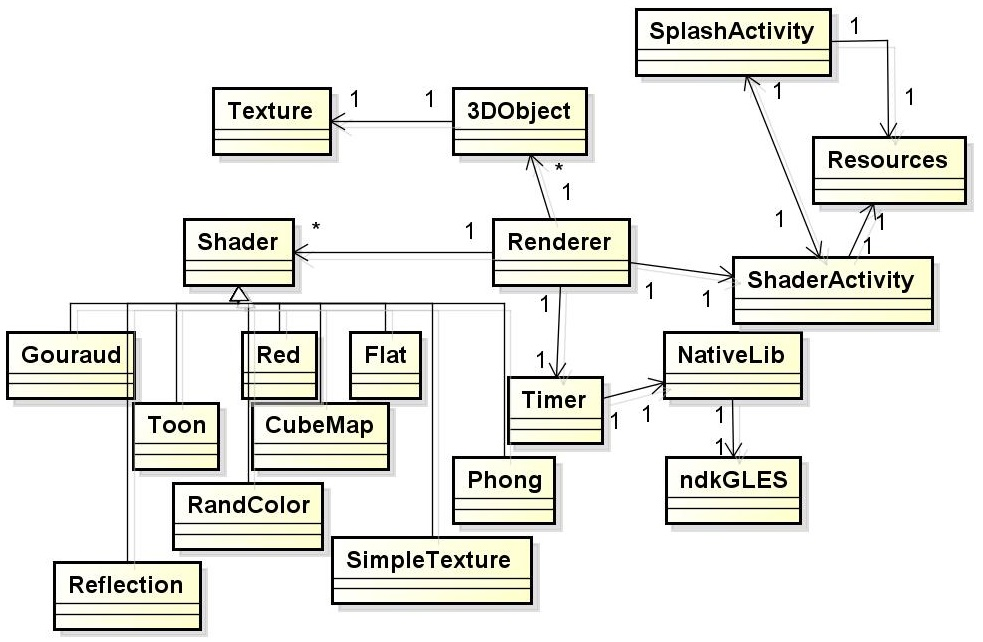
\includegraphics[keepaspectratio=true,scale=0.32]{class_diagram.jpg}
	\caption{Android implementation: class diagram}
	\label{class_diagram}
	\end{figure}

\subsubsection{Front-end Screen}

The front-end screen is responsible for the interaction with the user, 
passing the input information to the back-end. The Android platform
uses the term Activity to describe the application's front-end screen. It has 
design elements like text, buttons, graphics, among others. In this work,
there are two Activity classes: Shader Activity and Splash Activity (Fig. \ref{shader_splash}).

	\begin{figure}[!t]
	\centering
		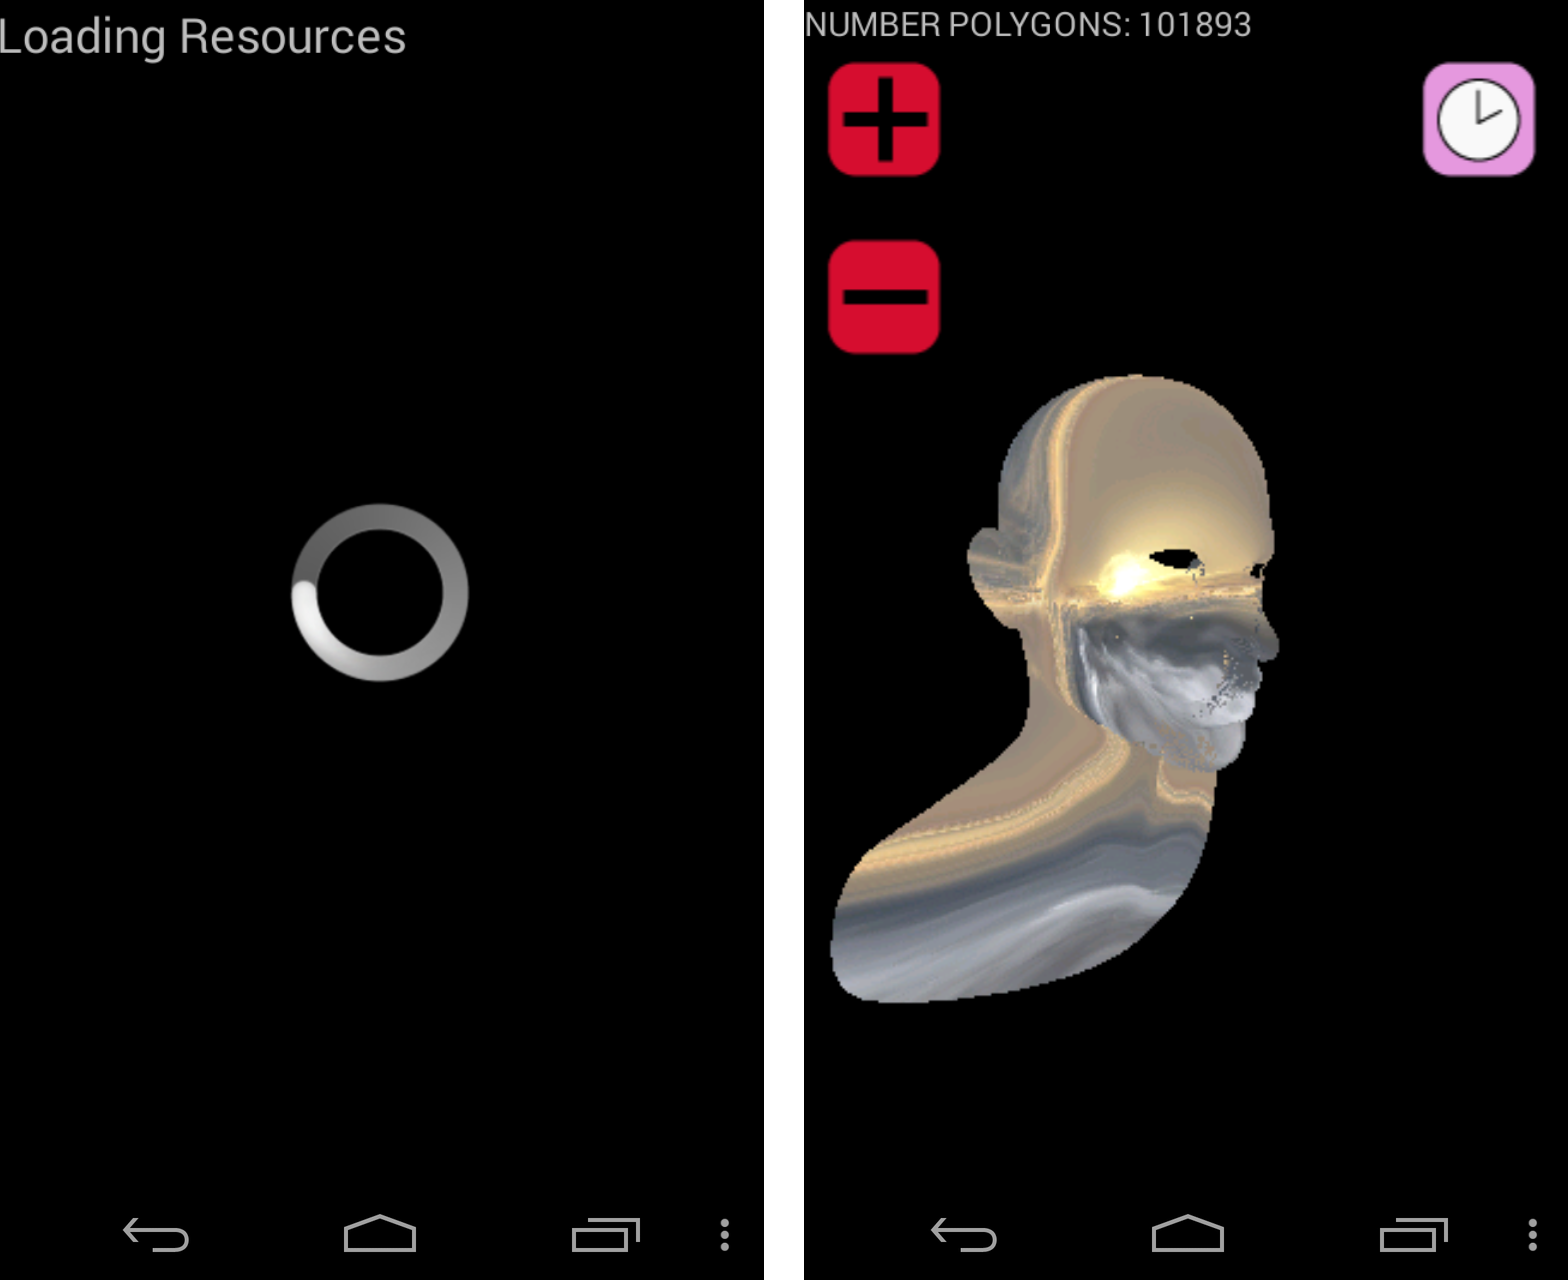
\includegraphics[keepaspectratio=true,scale=0.12]{shader_splash.png}
	\caption{Shader Activity and Splash Activity}
	\label{shader_splash}
	\end{figure}
	
 The Splash Activity is responsible for the visualization of the loading screen
while the necessary resources -- like the three-dimensional objects and textures --
are loaded by a thread. This resources are managed by the Resources class, that
uses the project pattern called Singleton. This pattern ensures that there's
only one instance class, which will be accessed later. 

 The Shader Activity is responsible for creating an instance of the Renderer 
class, which renders the three-dimensional objects. Besides, it controls the
touch events, that allows scaling and rotating these objects. It also shows
the buttons that increase and decrease the number of polygons.  

\subsubsection{Three-dimensional Object}

The three-dimensional object is represented by the composition of the 3DObject and
Texture classes. The 3DObject class is responsible for reading and interpreting the
obj files, that contains the information about the object. After this, the position, 
normal and texture vertices are stored into a buffer. The Texture class generates the textures, used by some shaders, from images.
Those images are created for each three-dimensional model, using the UV Mapping 
technique. It maps the texture coordinates to an image.

\subsubsection{Renderer}
	
The Renderer class works like a controller, being responsible for the 
rendering. It is the main class for the calls from the view (Shader Activity)
and model (3DObject, Shader and Timer) classes. This class implements the 
functions from the OpenGL ES library called \texttt{onSurfaceCreated()}, 
\texttt{onDrawFrame()} and \texttt{onSurfaceChanged()}.

\subsubsection{Shader}

The Shader class reads, attaches and links the vertex and fragment shaders.
Furthermore, it has the abstract methods \texttt{getParamsLocation()} and
\texttt{initShaderParams(Hashtable params)}. The first method stores the 
location of each variable specified in the shader. The second method initializes
these variables based on a hash, which contains the values for each variable. This way, 
every shader inherits from the Shader class and must implement these abstract methods.
The implemented shaders can be seen on Fig. \ref{shaders_impl}.

	\begin{figure}[!t]
	\centering
		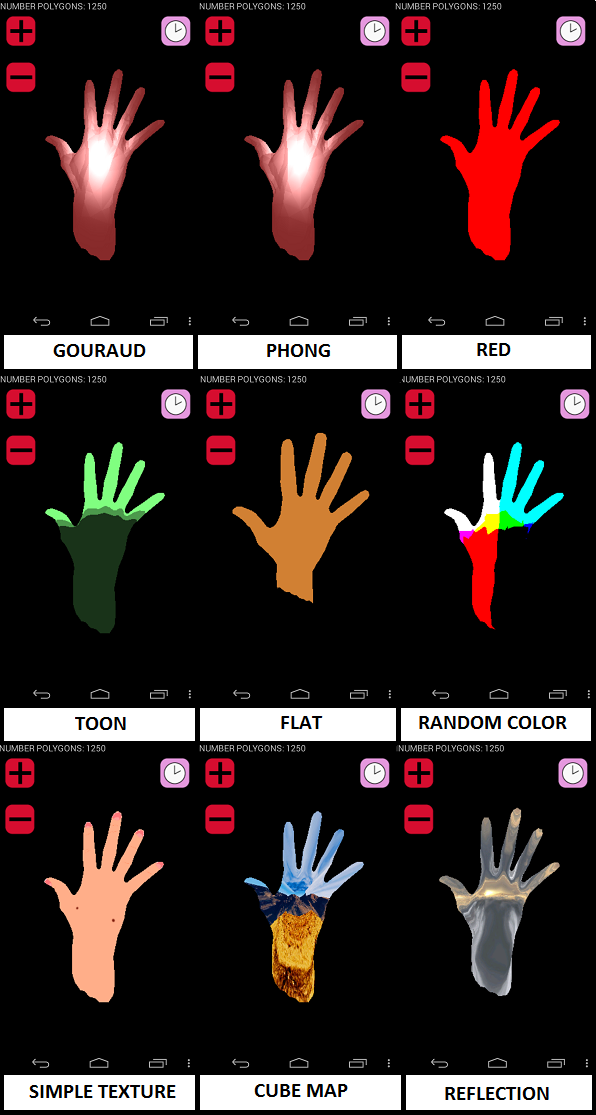
\includegraphics[keepaspectratio=true,scale=0.4]{shaders_impl.png}
	\caption{Implemented Shaders}
	\label{shaders_impl}
	\end{figure}

\subsubsection{Calculation of Rendering Time}
\label{time}
The Timer class measures the rendering time in nanoseconds. Each measurement is
done using the C language and the OpenGL ES extension called 
\texttt{GL\_EXT\_disjoint\_timer\_query}. The integration between the code in C 
language and the code in Java is done by the class called NativeLib. If the
extension is not available for the device, an alert is issued.

\subsection{iOS Implementation}
\label{sec:ios}

The structure of the code on iOS platform is similar to the Android, as is 
shown in Fig. \ref{ios_diag}. It follows the Model-View-Controller pattern, which the
controller is responsible for the integration between the Shader, 3DObject
classes and the view RendererView. 

	\begin{figure}[!t]
	\centering
		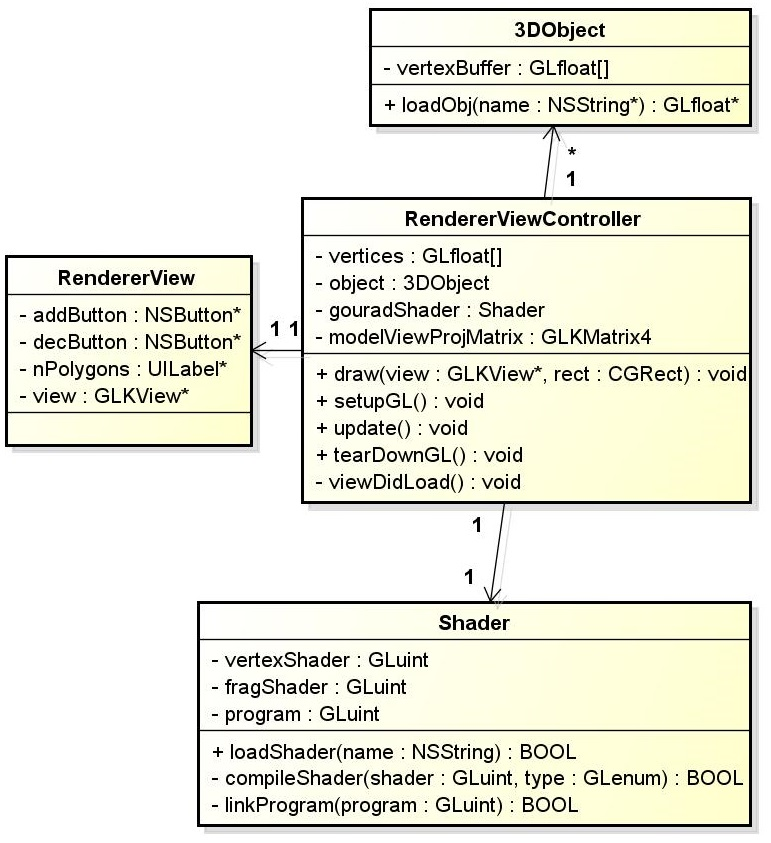
\includegraphics[keepaspectratio=true,scale=0.41]{ios_class_diagram.jpg}
	\caption{iOS implementation: class diagram}
	\label{ios_diag}
	\end{figure}

 The 3DObject class interprets the obj file to the format accepted by OpenGL ES. The Shader class, as in Android platform, reads, attaches and links the vertex
and fragment shaders. 

 The Gouraud Shader was chosen to be implemented and posteriorly to do the
comparisons between the different devices on distinct platforms. The result is seen on Fig. \ref{gouraud_ios}.

	\begin{figure}[!t]
	\centering
		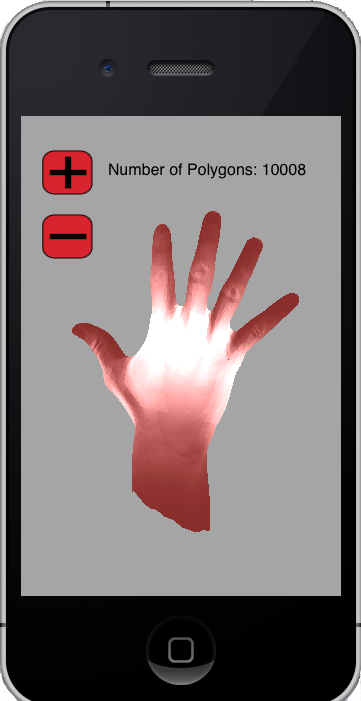
\includegraphics[keepaspectratio=true,scale=0.25]{gouraud_ios.png}
	\caption{Gouraud Shader on iOS platform }
	\label{gouraud_ios}
	\end{figure}
	
\subsection{Experimental Estimation of Asymptotic Complexity}
\label{sec:assy}

The experimental estimation of asymptotic complexity of each shader
was done by diverse measurements for each polygon counting (represented by each three-dimensional model). The
asymptotic complexity was analyzed by two points of view: related to the
entire rendering process and only related to the vertex and fragment shaders.

\subsubsection{Rendering Process}

In Android platform, as mentioned in Section \ref{time}, an OpenGL ES extension
was used to get the rendering process time, done by the \texttt{glDrawArrays()}
function. In iOS platform, the module -- from Xcode development tool -- called Instruments was used, 
which informs the elapsed time of each OpenGL ES function in microseconds.

 This way, the measures were gathered for the devices Nexus 4, iPhone 5s and
iPad Air. It wasn't possible to collect for the HTC One device, because the extension
wasn't available for this Android device.

\subsubsection{Vertex and Fragment Shaders}

The vertex and fragment shaders measurements were only possible to do in
Android devices. The reason is because the Instruments module of Xcode -- in iOS implementation -- doesn't exhibit
any information about them. Then, the tool used to collect the measures for Android devices was the
Adreno Profile, because the GPUs of these devices are Adreno. 

 The chosen metrics were instructions per second per vertex and instructions
per second per fragment. These metrics were gathered for each polygon counting,
being exported in CSV (Comma-Separated Values) format.

\subsubsection{Plot}

After the measurements were done, the charts were plotted both for the 
rendering process, as for the vertex and fragment shaders. The first set of charts is related to the time, 
in nanoseconds, versus the polygon count. The second is related to the number of instructions per second
per vertex (or fragment) versus the polygon count. 

\subsubsection{Automation of Curves Adjustments}

To do the curve adjustment, it was used the least squares method to linear,
quadratic, cubic and exponential functions. The squared errors associated to each
adjustment were also calculated, in order to determine which function had
a better approximation to the original measures. Smaller the error, the better the approximation.

 A program in Python was created to automate this calculation process. It reads
CSV or TXT files, calculates the average of the measures, plots the charts and
does the curve adjustment (also plotting the data). The program is command-line
based, having as parameters the shader name and the measurement used (if it's
related to the whole rendering process or just to the vertex and fragment shaders).

 The Listing \ref{linhacomando} shows two command-lines examples: the first is related
to the rendering process of the Gouraud shader and the second is related
only to the vertex and fragment shaders.

\lstinputlisting[language=C, numbers=none,label = {linhacomando}, caption = {Command-lines}]{linhacomando.txt}

 The Fig. \ref{python} shows how this program is structured.
The ReadCSV and ReadTxt classes are responsible for reading the CSV and TXT 
files. The PlotChart class plots the original and adjusted data and the 
LeastSquares calculates these adjustments and their errors.

	\begin{figure}[!t]
	\centering
		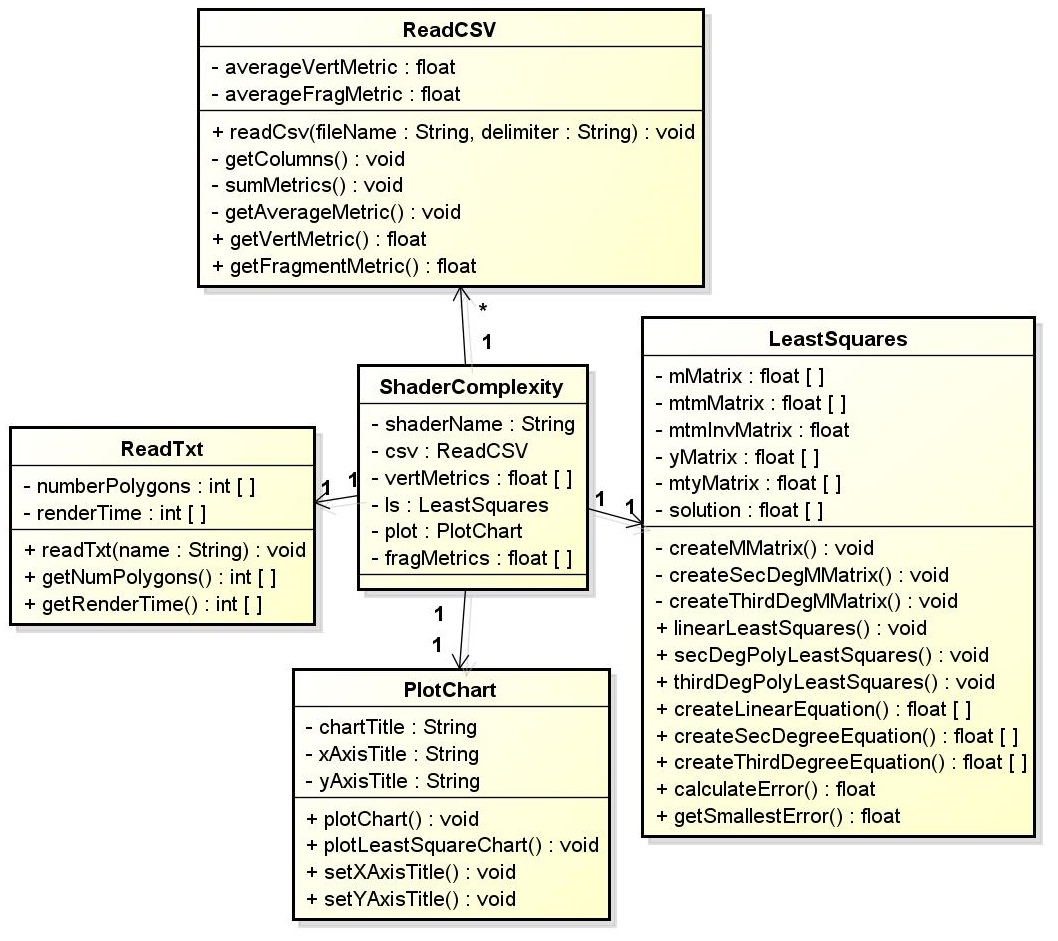
\includegraphics[keepaspectratio=true,scale=0.28]{minquad_diag.jpg}
	\caption{Tool implementation: class diagram}
	\label{python}
	\end{figure}

 In Fig. \ref{tool_result} the result of the tool for
the rendering process is presented, which is composed by four screens. 
The first one (top-down) is the plot of the linear adjustment, the second 
is the quadratic adjustment, the third is  the cubic  
adjustment and the last one is the exponential adjustment. 

	\begin{figure}[!t]
	\centering
		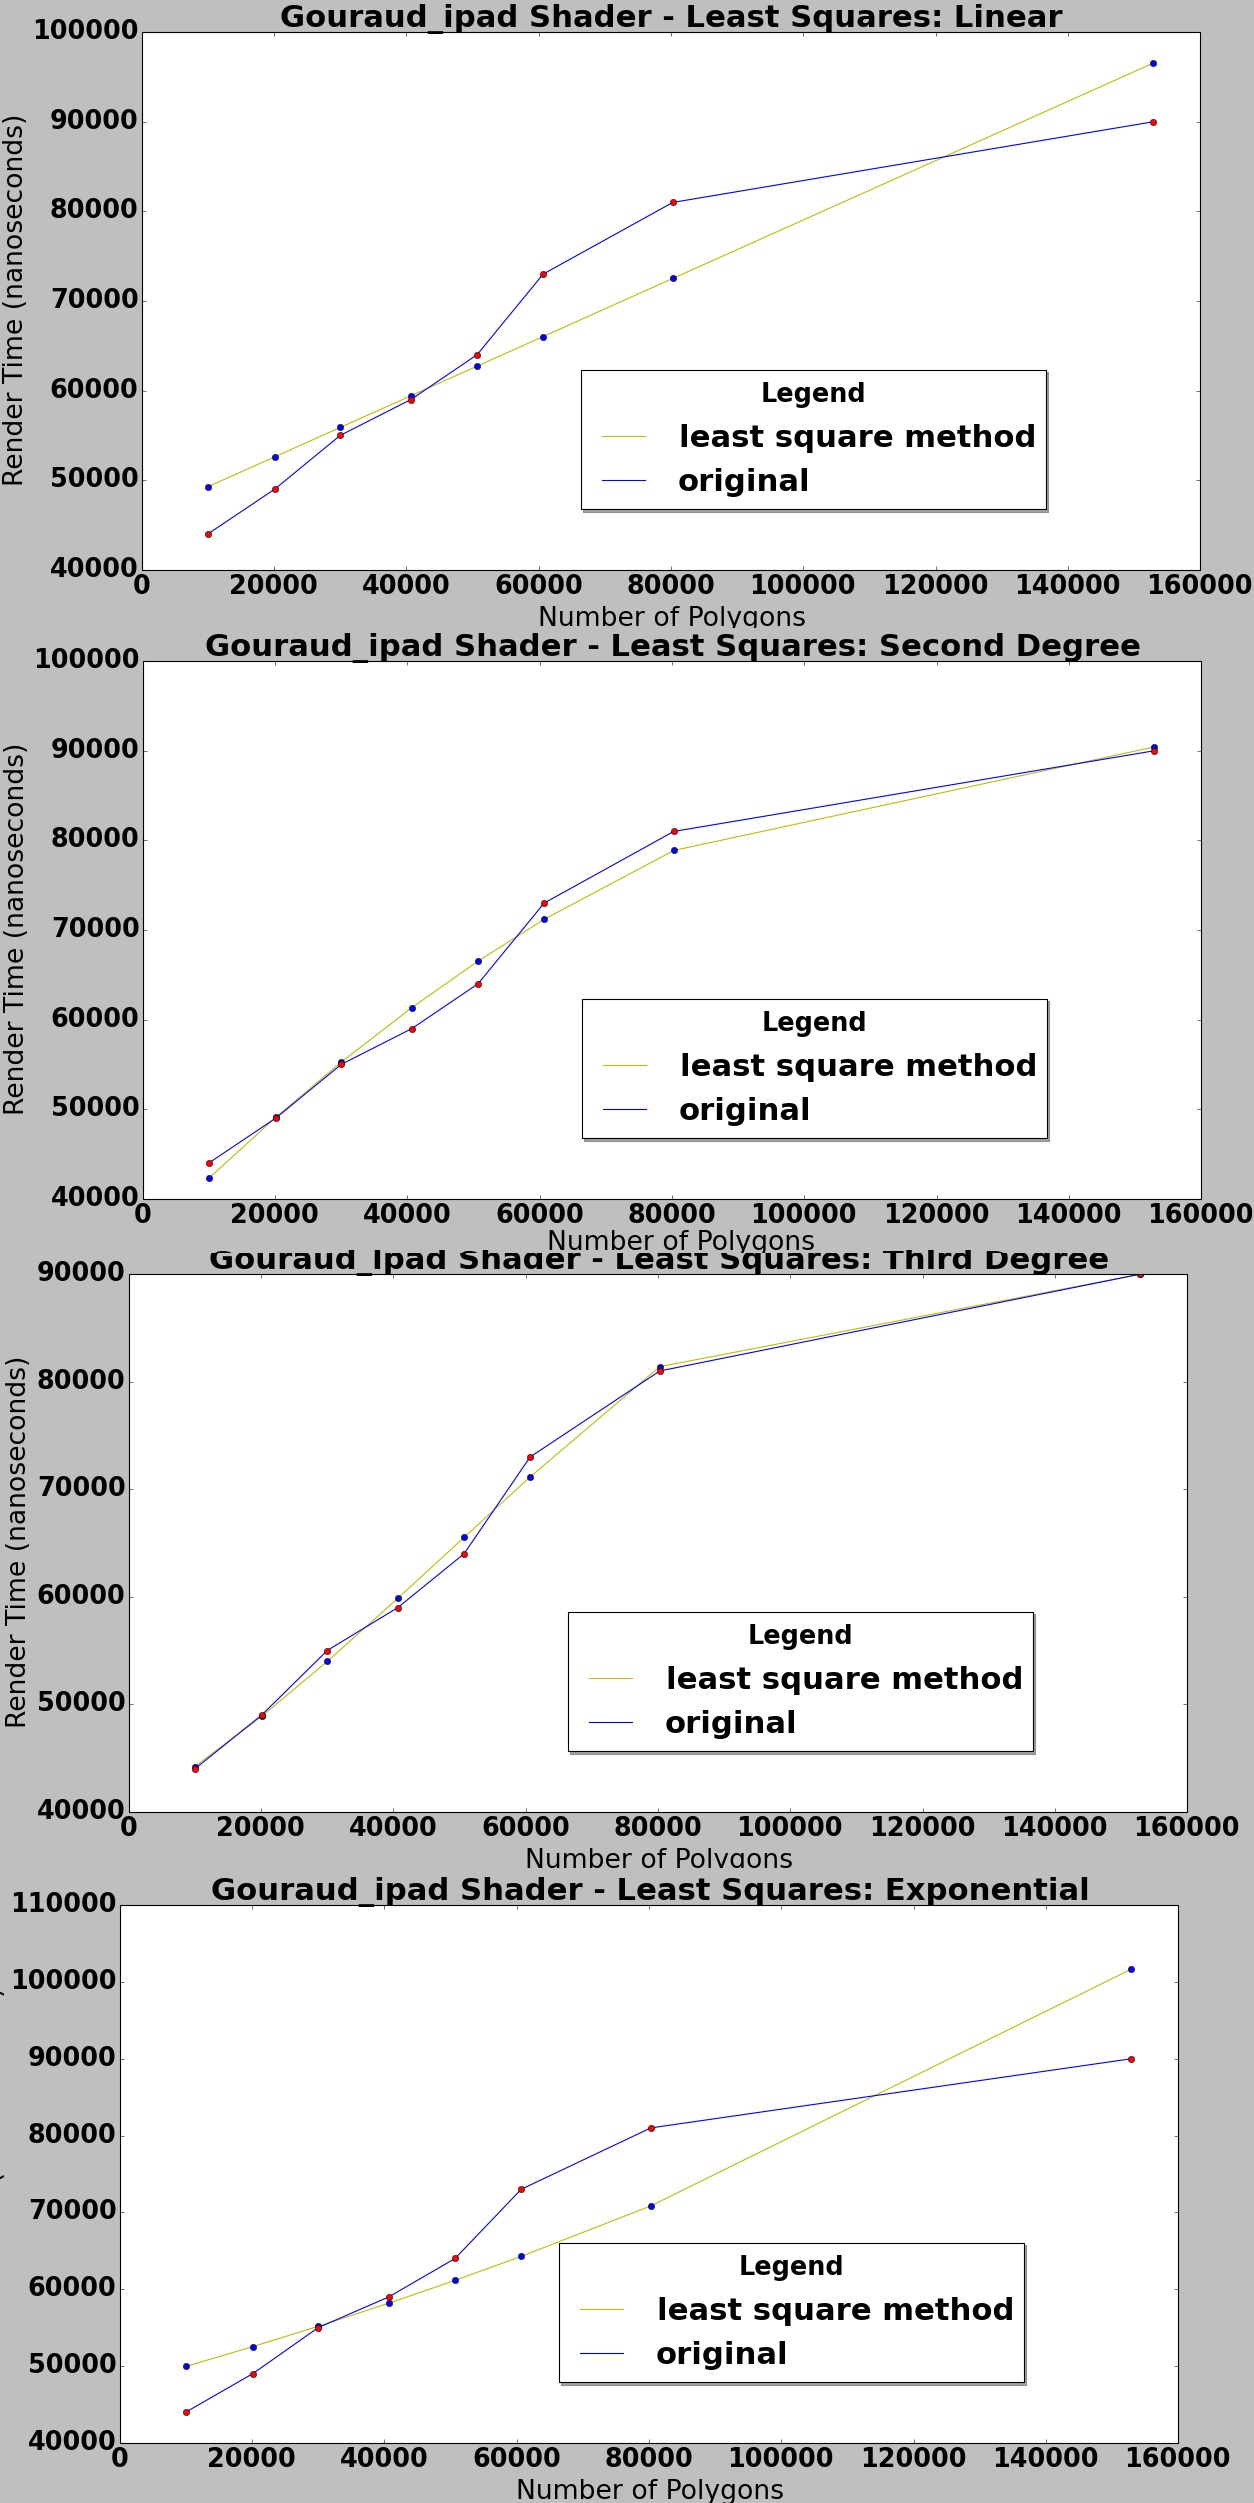
\includegraphics[keepaspectratio=true,scale=0.23]{ios_minquad_render.jpg}
	\caption{Automatic Adjustments: rendering process}
	\label{tool_result}
	\end{figure}

	
 In Fig. \ref{tool_result2} and Fig. \ref{tool_result3} the results of the tool for
the vertex and fragment shaders are presented, which are four screens with the adjustments as well.
At the end, the program shows the equations related to each adjustment
and their errors.

	\begin{figure}[!t]
	\centering
		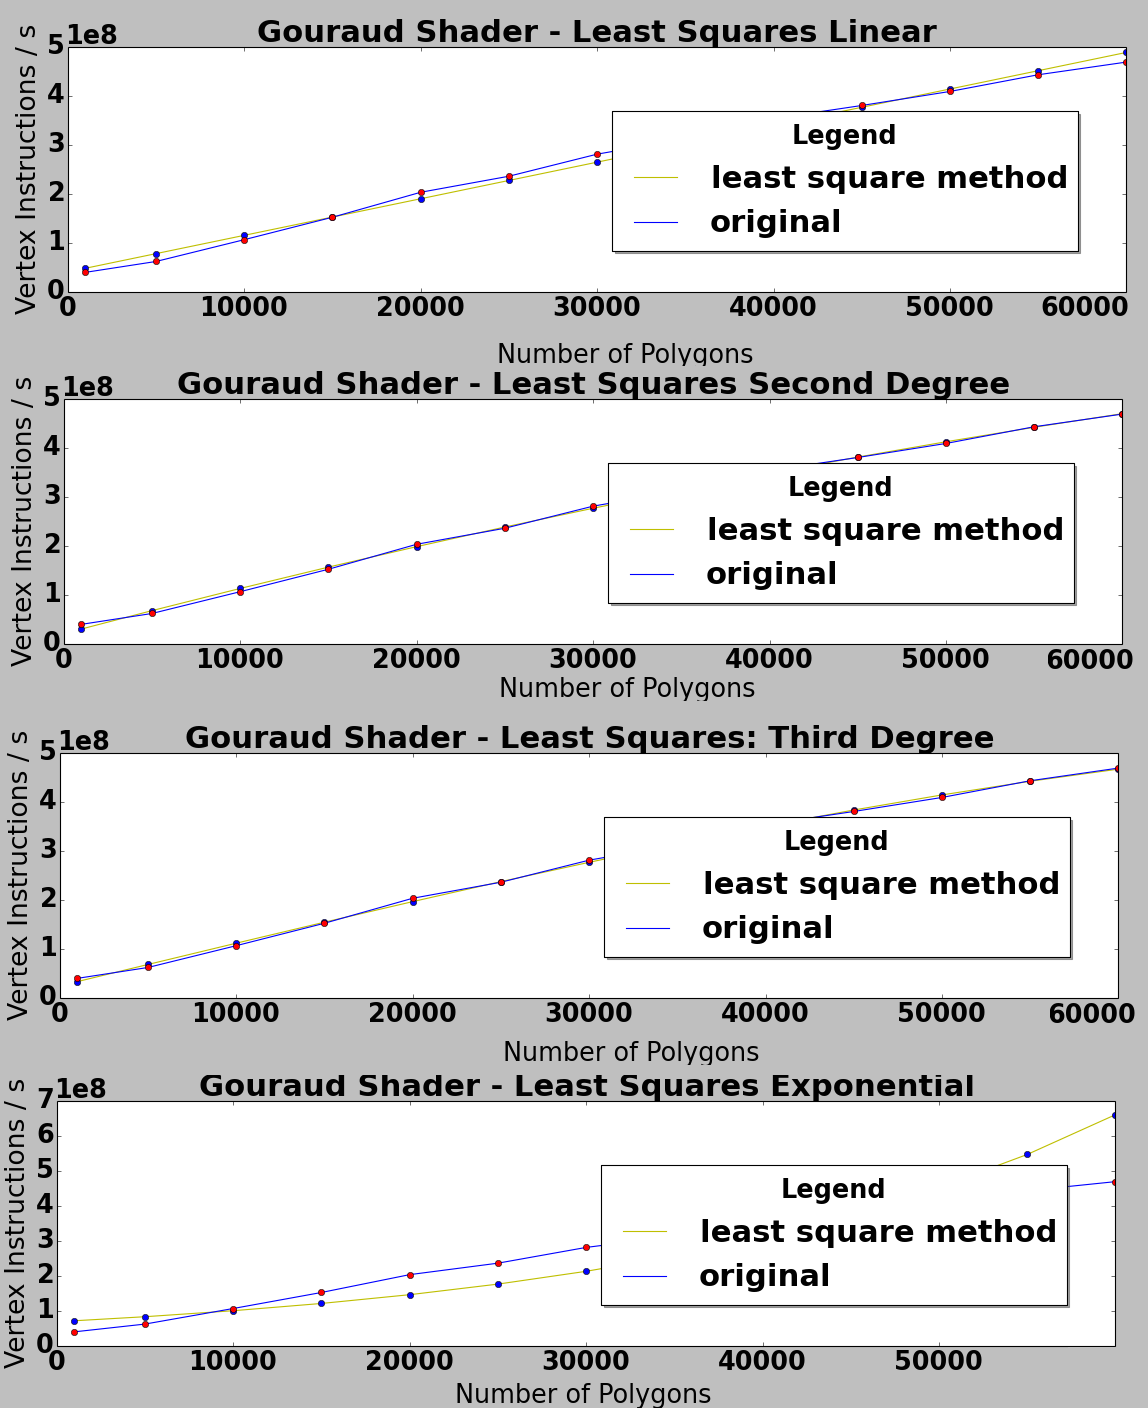
\includegraphics[keepaspectratio=true,scale=0.27]{vertex_minquad.png}
	\caption{Automatic Adjustments: vertex shader}
	\label{tool_result2}
	\end{figure}
	
	\begin{figure}[!t]
	\centering
		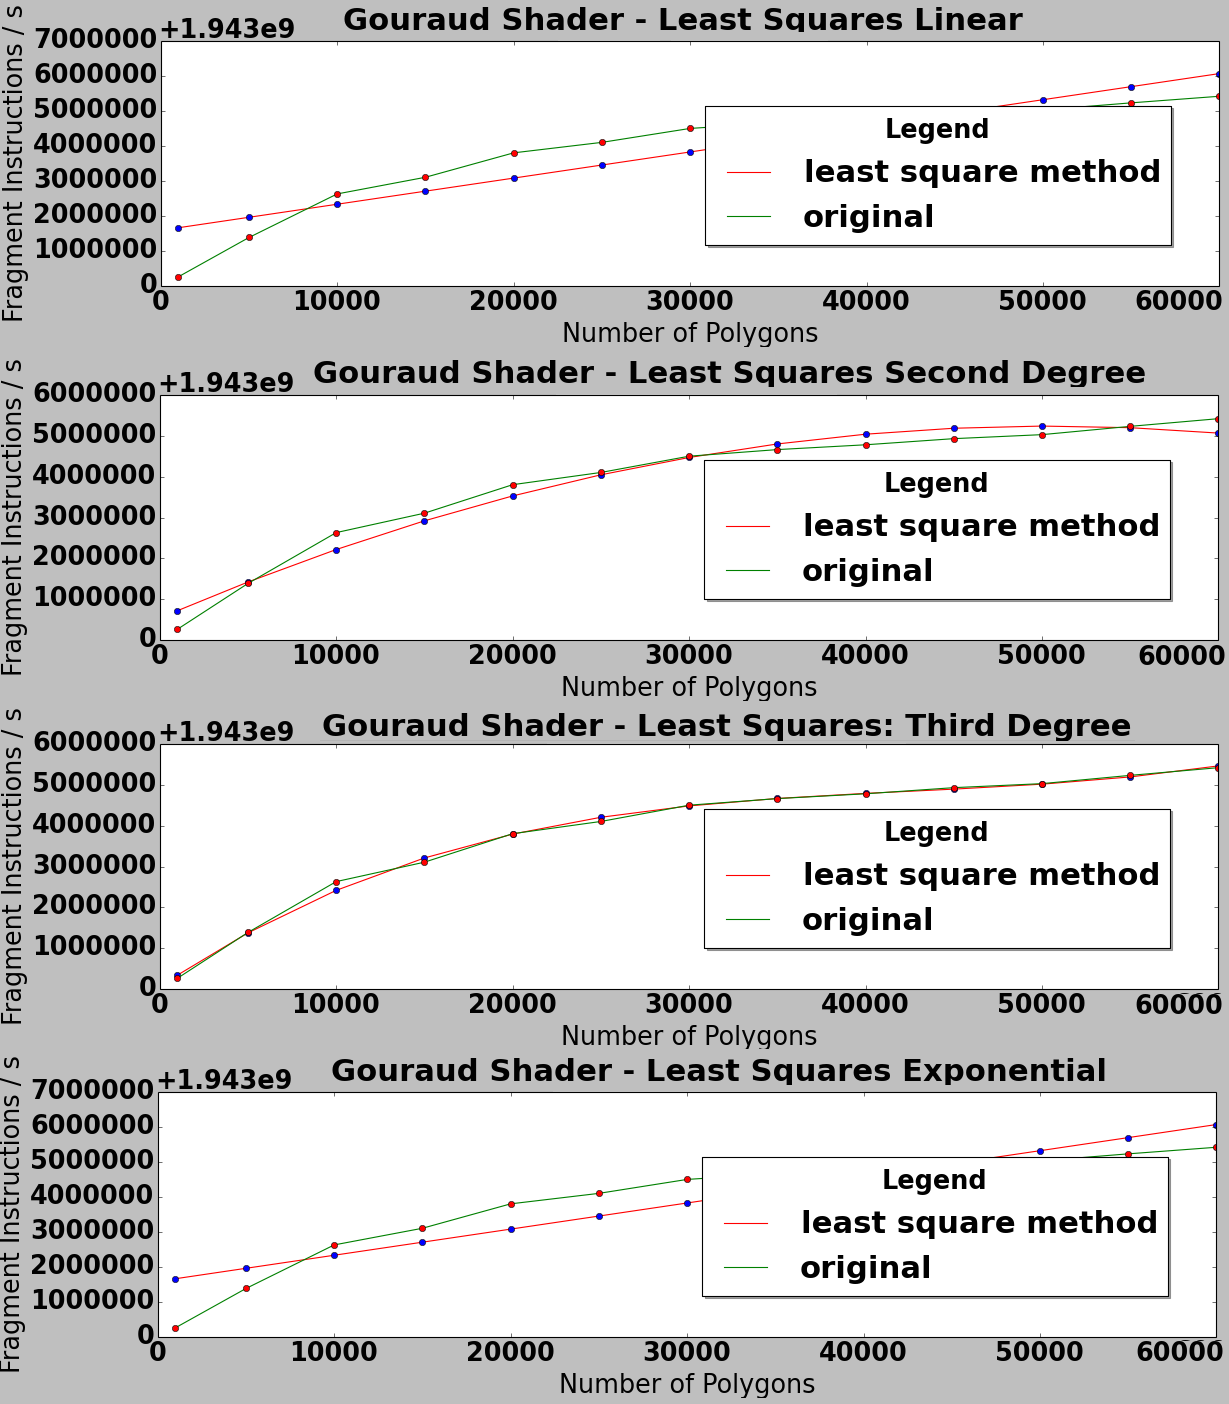
\includegraphics[keepaspectratio=true,scale=0.26]{fragment_minquad.png}
	\caption{Automatic Adjustments: fragment shader}
	\label{tool_result3}
	\end{figure}	
	

	
\section{Results}
\label{sec:generating-pdf-file}

For each shader were plotted the charts related to the entire rendering
process and to the vertex and fragment shaders for different devices.
After these plots, it was noticed that the charts for all shaders and devices
had similar curves for each measure type (rendering process, vertex and fragment shader).  

\subsection{Android Devices}

With the Nexus 4 device was possible to plot the charts related to the rendering
process and to the vertex and fragment shaders. The charts about the 
vertex shader visually resulted in a linear function (with different slopes).
The Fig. \ref{vertex_all} shows the charts related to the vertex shader of all implemented shaders.

	\begin{figure}[!t]
	\centering
		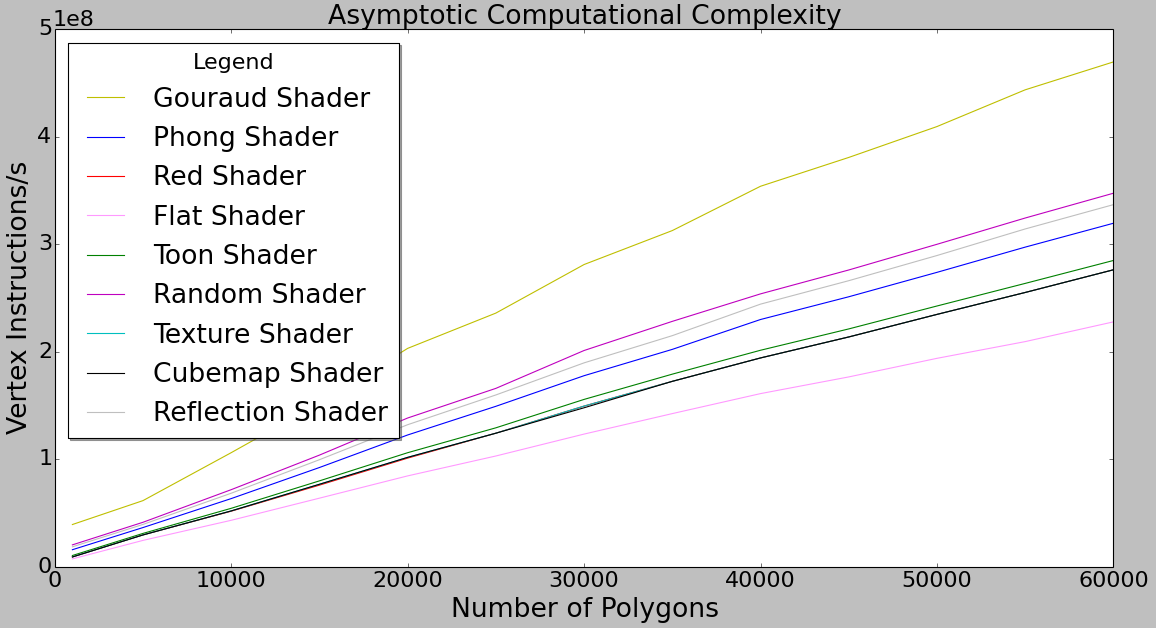
\includegraphics[keepaspectratio=true,scale=0.27]{vertex_all.png}
	\caption{Vertex shader: curves comparison}
	\label{vertex_all}
	\end{figure}
	
 The curves related to the rendering process and to the fragment shader had similar shapes,
but it wasn't possible to determine the exact curve only by visual
inspection. These curves are shown in the Fig. \ref{fragment_all} and Fig. \ref{render_all}. 

	\begin{figure}[!t]
	\centering
		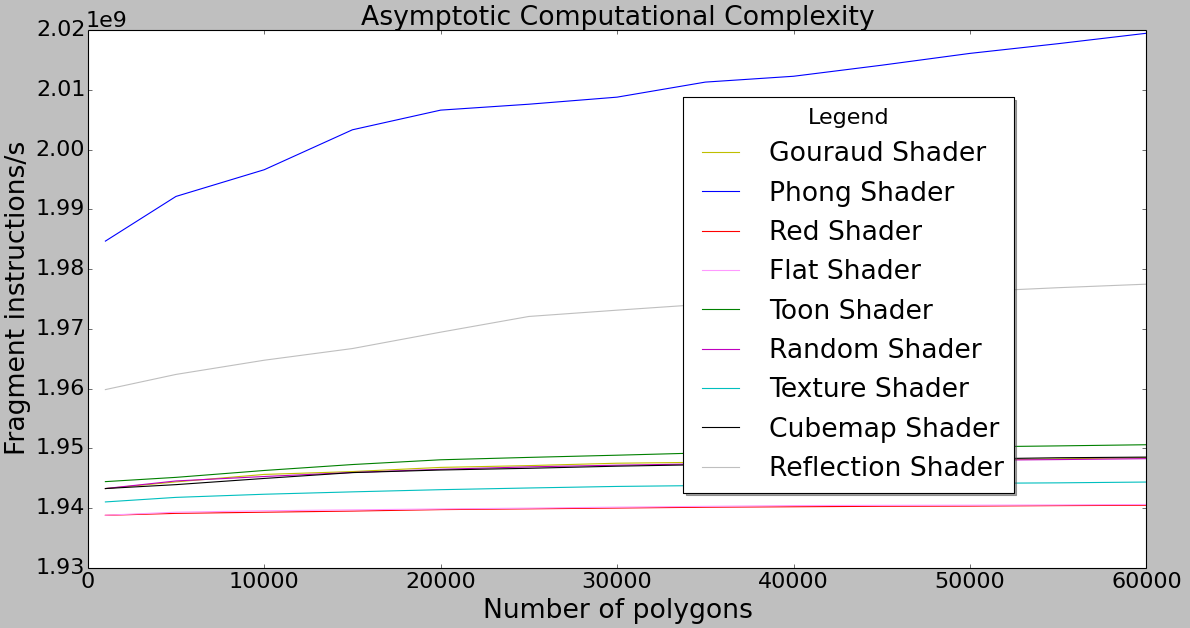
\includegraphics[keepaspectratio=true,scale=0.22]{fragment_all.png}
	\caption{Fragment shader: curves comparison}
	\label{fragment_all}
	\end{figure}
	
	\begin{figure}[!t]
	\centering
		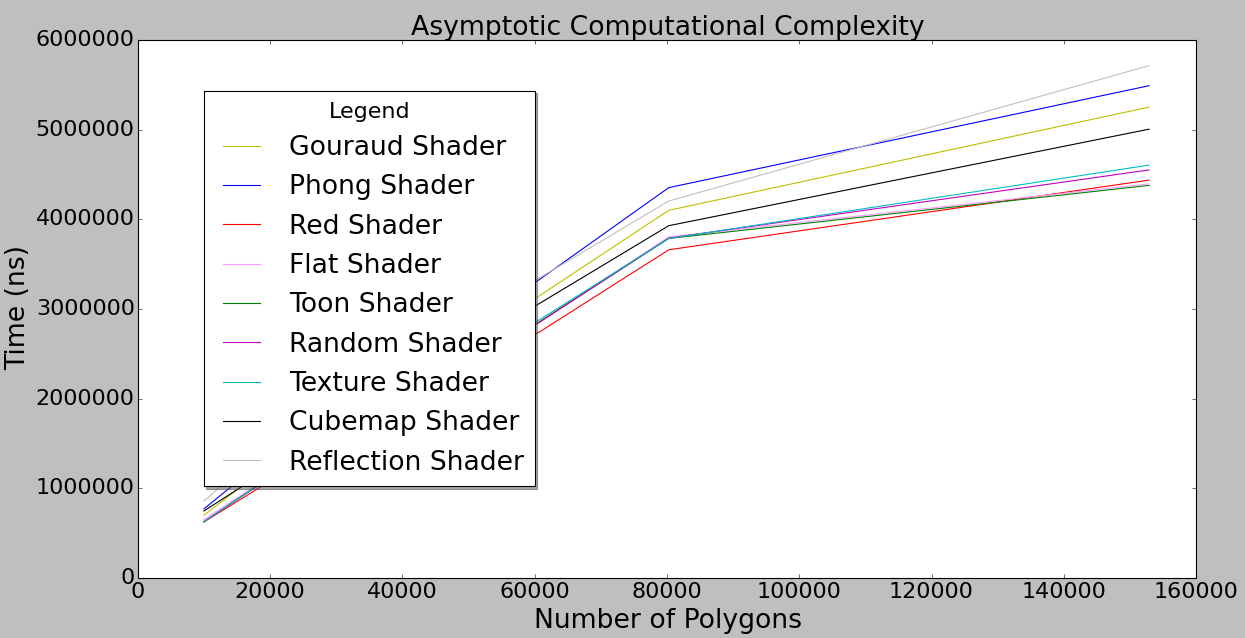
\includegraphics[keepaspectratio=true,scale=0.25]{render_time_all.png}
	\caption{Rendering process: curves comparison}
	\label{render_all}
	\end{figure}
	
 Then, the adjustments to the predefined curves were done by the automated tool
and plotted for each shader. The smallest errors were also determined, in order
to discover which curve had the best approximation. By this analysis, all the shaders had better 
approximation to a third degree curve, both for the fragment shader as for the rendering process.

 For the HTC One device was only possible to measure the performance
related to the vertex and fragment shader. The results were the same as
in the Nexus 4, which the vertex shader had a linear behavior and 
the fragment shader, a cubic behavior (Fig. \ref{htc_one}). 

	\begin{figure}[!t]
	\centering
		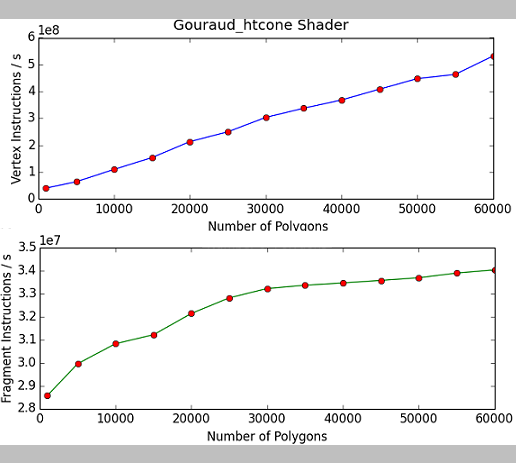
\includegraphics[keepaspectratio=true,scale=0.6]{htc_render.png}
	\caption{HTC One device}
	\label{htc_one}
	\end{figure}
	
\subsection{iOS Devices}

With the iOS devices, it was only possible to plot the charts related
to the rendering process. The shapes of the obtained curves are
similar to the obtained curves in Nexus 4, and the best approximations
were also to a third degree curve. The Fig. \ref{ios_devices} shows these curves 
for the iPhone 5s and for the iPad Air.

	\begin{figure}[!t]
	\centering
		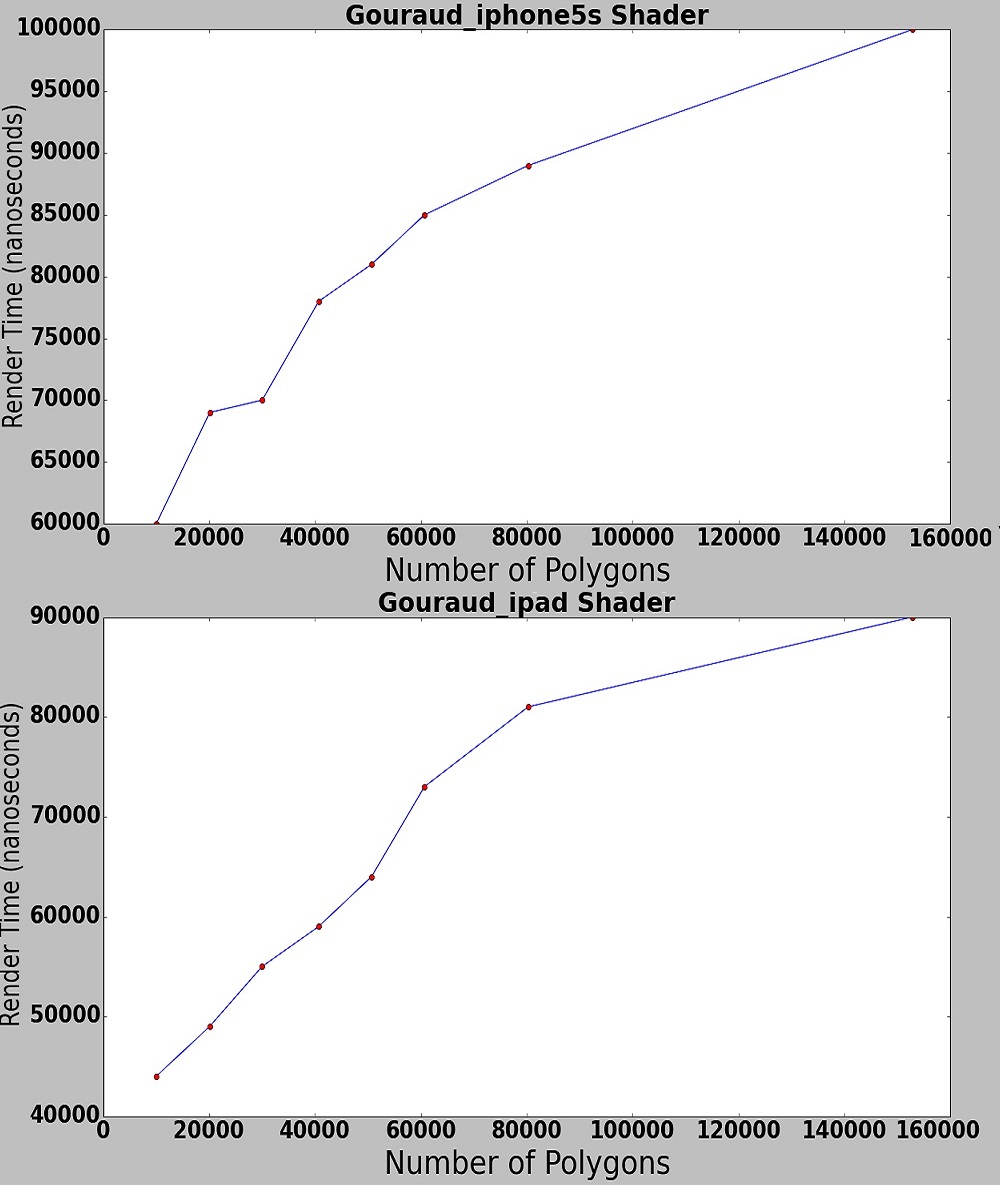
\includegraphics[keepaspectratio=true,scale=0.27]{ios_render_time.jpg}
	\caption{iOS devices}
	\label{ios_devices}
	\end{figure}

\subsection{Analysis of the Equations}

With the automated tool, it was also possible to calculate the equations
of the adjusted curves, for each shader of the 
Nexus 4. They are shown in Table \ref{equation_nexus_vertex}, Table \ref{equation_nexus_fragment} and
Table \ref{eqrender}. Although the 
curves are of the same family, their coefficients are not identical.
The shaders relatively more complexes had steeper slopes 
compared to the simple shaders and they had greater $x^2$ and $x^3$ coefficients. 

\begin{table}[!t]
\centering
\caption{Equations related to the vertex shader}
\begin{tabular}{ll}
	\hline
	\textbf{Shader Name} & \textbf{Vertex Instructions per Second} \\
	\hline
	Gouraud & $y = 40.16 \times 10^6 + 7486.43n$  \\
	Phong &  $y = 14.95 \times 10^6 + 5211.02n$  \\
	Red & $y = 8.02 \times 10^6 + 4545.69n$ \\
	Toon & $y = 10.17 \times 10^6 + 4673.96n$ \\
	Flat & $y = 7.65 \times 10^6 + 3738.61n$ \\
	Random Color & $y = 20.58 \times 10^6 + 5640.13n$ \\
	Simple Texture & $y = 8.80 \times 10^6 + 4540.32n$ \\
	CubeMap & $y = 8.67 \times 10^6 + 4540.40n$ \\
	Reflection & $y = 18.03 \times 10^6 + 5470.95n$ \\
	\hline
\end{tabular}
\label{equation_nexus_vertex}
\end{table}

\begin{table}[!t]
\caption{Equations related to the fragment shader}
\centering
\begin{tabular}{ll}
	\hline
	\textbf{Shader Name} & \textbf{Fragment Instructions per Second}  \\
	\hline
	Gouraud & \begin{tabular}{@{}l@{}}$y = 19.43 \times 10 ^8 + 297.00n $ \\ $- 0.0065n^2 + 0.50 \times 10^{-7}n^3 $\end{tabular}\\ [2ex]
	Phong  & \begin{tabular}{@{}l@{}}$y = 19.84 \times 10^8 + 1752.43n $ \\ $- 0.0389n^2 + 3.32 \times 10^{-7}n^3$ \end{tabular}  \\ [2ex]
	Red &  \begin{tabular}{@{}l@{}}$y = 19.39 \times 10 ^8 + 64.34n $ \\ $- 0.00090n^2 + 0.05 \times 10^{-7}n^3$\end{tabular}\\ [2ex]
	Toon & \begin{tabular}{@{}l@{}}$y = 19.44 \times 10 ^8 + 268.89n $ \\ $- 0.0044n^2 + 0.30 \times 10^{-7}n^3$\end{tabular} \\ [2ex]
	Flat & \begin{tabular}{@{}l@{}}$y = 19.39 \times 10 ^8 + 74.94n $ \\ $- 0.0013n^2 + 0.08 \times 10^{-7}n^3$\end{tabular} \\ [2ex]
	Random Color & \begin{tabular}{@{}l@{}}$y = 19.43 \times 10 ^8 + 250.33n $ \\ $- 0.0050n^2 + 0.37 \times 10^{-7}n^3$\end{tabular} \\ [2ex]
	Simple Texture & \begin{tabular}{@{}l@{}}$y = 19.41 \times 10 ^8 + 160.00n $ \\ $- 0.0030n^2 + 0.22 \times 10^{-7}n^3$\end{tabular}\\ [2ex]
	CubeMap & \begin{tabular}{@{}l@{}}$y = 19.43 \times 10 ^8 + 245.89n $ \\ $- 0.0047n^2 + 0.37 \times 10^{-7}n^3$\end{tabular} \\ [2ex]
	Reflection & \begin{tabular}{@{}l@{}}$y = 19.59 \times 10 ^8 + 698.57n $ \\ $- 0.0094n^2 + 0.47 \times 10^{-7}n^3$\end{tabular} \\ [2ex]

	\hline
\end{tabular}
\label{equation_nexus_fragment}
\end{table}

\begin{table}[!t]
\centering
\caption{Equations related to the rendering process}	
\begin{tabular}{ll}
	\hline
	\textbf{Shader Name} & \textbf{Rendering Process Time (ns)}  \\
	\hline
	Gouraud & \begin{tabular}{@{}l@{}l@{}}$y = 24.31 \times 10^4 + 48.89n + 7,60 $ \\  $\times 10^{-5}n^2 - 1.19 \times 10^{-9}n^3$\end{tabular}  \\[2ex]
	Phong & \begin{tabular}{@{}l@{}l@{}}$y = 31.25 \times 10^4 + 49.28n + 0.12 $ \\ $\times 10^{-5}n^2 - 1.43 \times 10^{-9}n^3$\end{tabular}\\[2ex]
	Red &  \begin{tabular}{@{}l@{}}$y = 30.37 \times 10^4 + 32.92n + 0.26 $ \\ $\times 10^{-5}n^2 - 0.00019 \times 10^{-9}n^3$\end{tabular} \\[2ex]
	Toon &  \begin{tabular}{@{}l@{}}$y = 27.28 \times 10^4 + 37.30n + 0.23 $ \\ $\times 10^{-5}n^2 - 1.93 \times 10^{-9}n^3$\end{tabular} \\[2ex]
	Flat &  \begin{tabular}{@{}l@{}}$y = 32.82 \times 10^4 + 33.84n + 0.28 $\\ $\times 10^{-5}n^2  - 2.15 \times 10^{-9}n^3$\end{tabular} \\[2ex]
	Random Color & \begin{tabular}{@{}l@{}}$y = 26.25 \times 10^4 + 38.42n + 0,20 $ \\ $\times 10^{-5}n^2 - 1.76 \times 10^{-9}n^3$\end{tabular} \\[2ex]
	Simple Texture & \begin{tabular}{@{}l@{}}$y = 24.51 \times 10^4 + 38.88n + 0,18 $\\ $\times 10^{-5}n^2 - 1.65 \times 10^{-9}n^3$\end{tabular} \\[2ex]
	CubeMap & \begin{tabular}{@{}l@{}}$y = 29.87 \times 10^4 + 44.70n + 0.11 $ \\ $\times 10^{-5}n^2 - 1.28 \times 10^{-9}n^3$\end{tabular}\\[2ex]
	Reflection & \begin{tabular}{@{}l@{}}$y = 33.63 \times 10^4 + 57.31n - 9.18 $ \\ $\times 10^{-5}n^2 - 0.35\times 10^{-9}n^3$ \end{tabular}\\[2ex]
	\hline
\end{tabular}
\label{eqrender}
\end{table}

 Analyzing the equations, it's possible to see that the vertex shader that
had better performance was the Flat Shader, which only determines the 
$x$ and $y$ coordinates (since the $z$ is zero). The vertex shader that had worst performance was the 
Gouraud Shader, which calculates the light components in the vertex shader.

 The shader with better performance -- related to the fragment shader -- was
the Red Shader, in which only determines the fragment color to red. The fragment shader with worst performance was the Phong Shader, which
does the same calculation as the Gouraud shading but in the fragment shader
instead of the vertex shader.

 The shaders with better performance -- related to the rendering process -- 
were the Flat, Toon and Red Shaders. The shaders with worst performance were 
the Reflection and Gouraud Shaders.

 Besides, with the equations, it's possible to estimate
the number of vertex or fragment instructions per second. Taking the Toon
Shader as example, which its vertex shader equation is 
$y(n) = 10.17 \times 10^6 + 4673.96n$, the estimated number of instructions 
per second for 60,000 polygons is $29.06 \times 10^7$. With the tool Adreno 
Profiler it was possible to see that this value is close
to the measured ($28.49 \times 10^7$).

 Another relevant result is about the Gouraud and Phong Shaders. The first had
the worst vertex shader performance and the second had the worst fragment 
shader performance. But the shader that had the worst rendering process 
performance was the Phong Shader. This result is consistent because the
fragment shader, by this experiment, has asymptotic complexity $O(n^3)$ and
the vertex shader, $O(n)$, influencing this worst outcome.

\subsubsection{Devices Comparison}

With the obtained curves and equations, it was also possible to compare
the devices. The Fig. \ref{nexus_htc_vertex} and Fig. \ref{nexus_htc_fragment} 
shows the curves related to the
vertex and fragment shaders for the Nexus 4 and HTC One devices. The
Fig. \ref{nexus_ios} compares the shaders related to the rendering process
for the Nexus 4 and the iOS devices.

	\begin{figure}[!t]
	\centering
		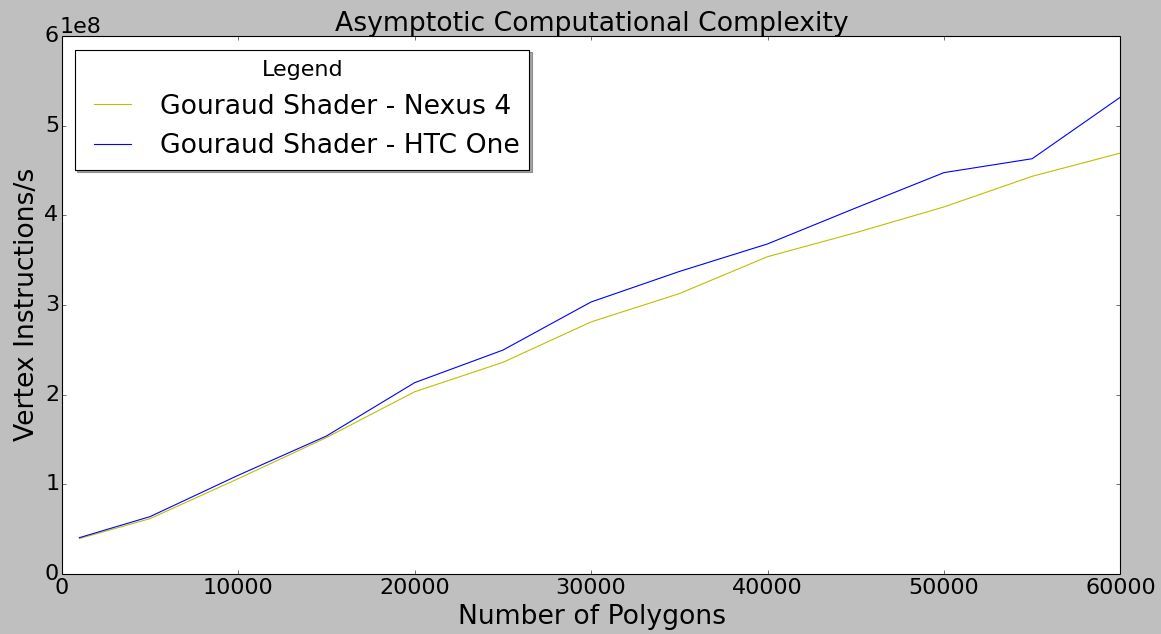
\includegraphics[keepaspectratio=true,scale=0.27]{vertex_devices_all.png}
	\caption{Nexus 4 and HTC One comparison: vertex shader}
	\label{nexus_htc_vertex}
	\end{figure}
	
	\begin{figure}[!t]
	\centering
		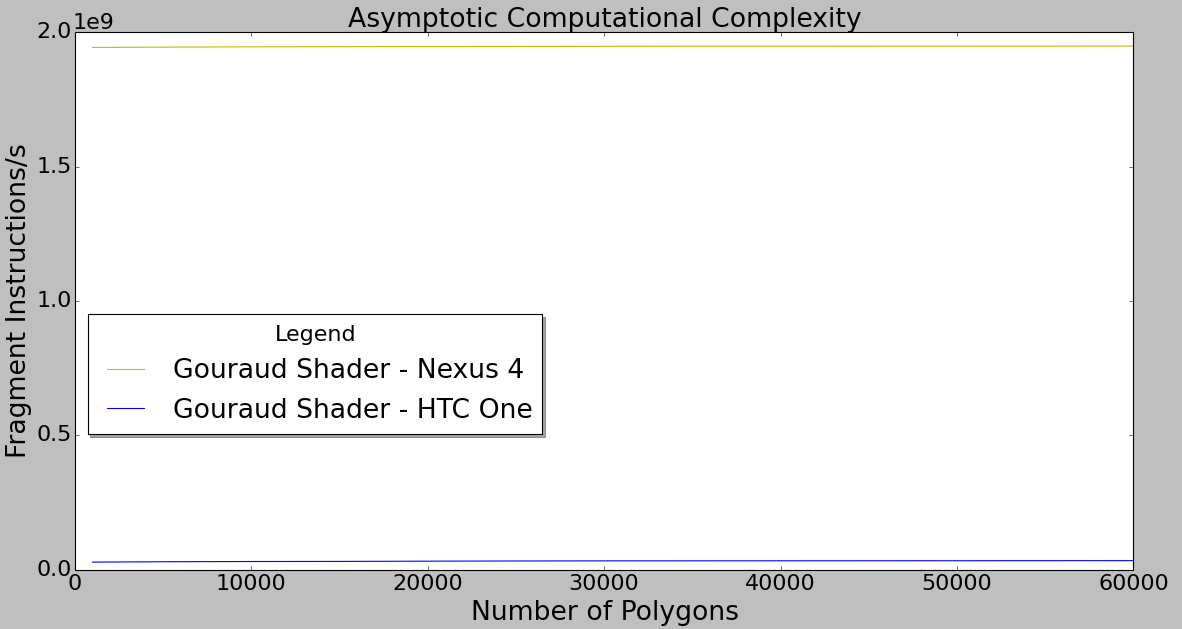
\includegraphics[keepaspectratio=true,scale=0.27]{fragment_devices_all.png}
	\caption{Nexus 4 and HTC One comparison: fragment shader}
	\label{nexus_htc_fragment}
	\end{figure}
	
	\begin{figure}[!t]
	\centering
		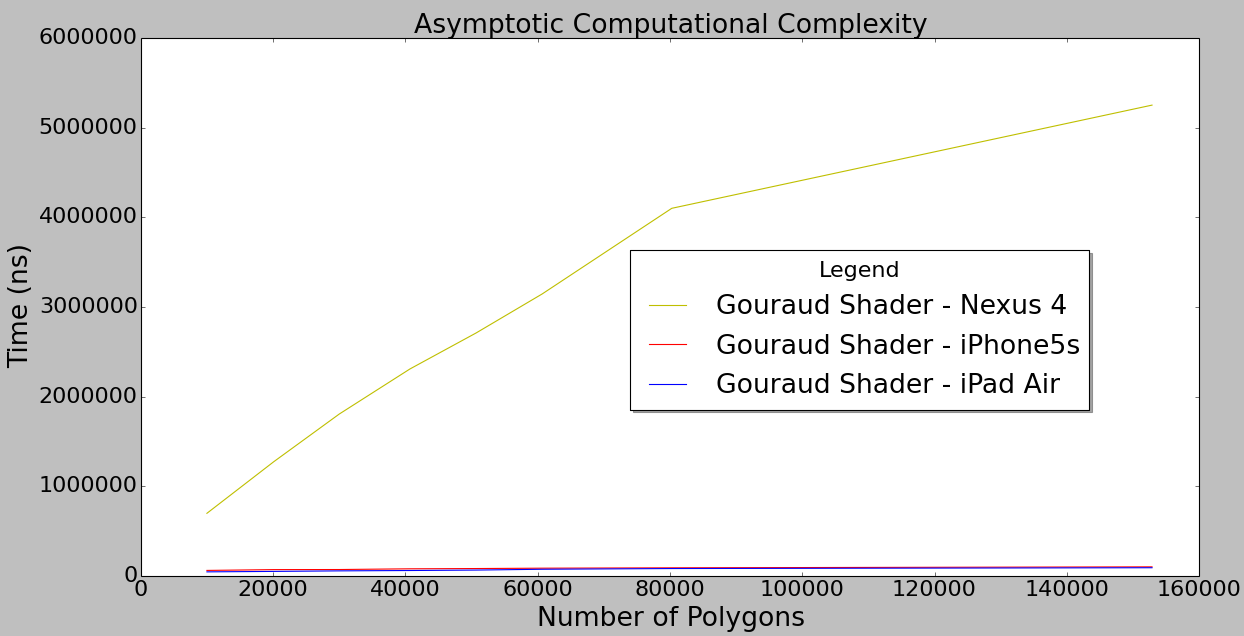
\includegraphics[keepaspectratio=true,scale=0.25]{render_time_devices.png}
	\caption{Nexus 4, iPhone 5s and iPad comparison: rendering process}
	\label{nexus_ios}
	\end{figure}	

 By the measurements and obtained equations, the device that had better
performance, related to the rendering process, was the iPad Air, which is
the device with better hardware configuration. And as it was shown in 
Section \ref{equip}, the iPad Air was the device with better position in 
the benchmark app. The device with worst performance was the Nexus 4 and 
this is consistent because it has the worst hardware configuration.

For the vertex shader, the Nexus 4 had better performance than the HTC One.
On the other hand, for the fragment shader, the HTC one had better performance
than the Nexus 4.

\subsubsection{Final Thoughts About the Equations}

Through the results, it was revealed that both rendering process and fragment
shader tended to present as asymptotic complexity a third degree function
for any shader. However, even that the squared errors were smallest to a third degree function,
the coefficients related to the $n^3$ term are very small, being of the 
order $10^{-7}$, $10^{-8}$ and $10^{-9}$. In case of $10^{-7}$, by example, it will be added or subtracted one unit
for each 100 million units of $n$ (for a $y(n)$ function), 
which can be considered irrelevant.

 This way, the curve related to the second degree function, even with 
bigger squared error, represents the reality of the shader better than the
third degree function. Then, the asymptotic complexity of the fragment 
shader and of the rendering process can be considered $O(n^2)$. The analysis done to the third degree 
equations is still valid to the second degree equations.
\subsection{Estimates in Production Environments}

In the gaming industry, the metric commonly used to determine the 
performance of a game is the FPS (Frames Per Second). This metric 
represents the number of images rendered per second. This way,
it's also possible to convert the obtained results in this work 
to this metric, like is shown in (\ref{fps_eq}),
where $t$ is the time in seconds (the metric used for the rendering process).

	\begin{equation}
		FPS = \frac{1} {t}
	\label{fps_eq}
	\end{equation}
	
It's also possible to obtain this time metric based on the number of instructions
per second (the metric used for the vertex and fragment shaders). Equation (\ref{fps_eq2}) shows how to do this conversion, in which is necessary
to use the tool Adreno Profiler to get the number of instructions for one
frame.

	\begin{equation}
		t = \frac{I_F} {I_S}
	\label{fps_eq2}
	\end{equation}
	where $I_{F}$ is the number of instructions for one frame and 
$I_{S}$  is the number of instructions per second.

Before converting the time metric to frames per second, for the rendering process,
it was added to the $t$ variable, the time spent by the other functions
in the OpenGL ES. These are the functions used for one frame in the draw call,
that doesn't vary with the number of polygons, like the function that sets the
background color, by example. 

In Android devices, these times were 
obtained with the same OpenGL ES extension used before. In iOS devices, they
were obtained with the Instruments tool, that informs the time spent by
each function.

The Table \ref{fps} presents the converted results in frames per second, 
taking the Gouraud Shader as example, for the Nexus 4 device. An important
observation is that these measures don't include the other factors present
in a real production environment, like input events and physics, by example.

	\begin{table}[!t]	
	\caption{Estimated FPS}
	\begin{tabular}{cccc}
		\hline
		\begin{tabular}{@{}c@{}}\textbf{Number} \\ \textbf{of Polygons}\end{tabular}
		& \begin{tabular}{@{}c@{}}\textbf{Time Spent (s):} \\ \textbf{\texttt{glDrawArrays}}\end{tabular} 
		& \begin{tabular}{@{}c@{}}\textbf{Time Spent (s):} \\ \textbf{Other Functions}\end{tabular}
		& \textbf{FPS}  \\
		\hline
		10,000 &  0.000698 &  0.0000140 & 1,405 \\
		20,100 &  0.00127 &  0.0000140 & 779 \\
		30,000 &  0.00181 &  0.0000140 & 548 \\
		40,678 &  0.00231 &  0.0000140 & 430 \\
		50,679 &  0.00271 &  0.0000140 & 367 \\
		60,662 &  0.00315  &  0.0000140 & 316 \\
		80,256 &  0.00410  &  0.0000140 & 243 \\
	          152,840 & 0.00525 &  0.0000140 & 190 \\
		\hline
	\end{tabular}
	
	\label{fps}
	\end{table}
	

\section{Discussion and Future Work}
\label{sec:discuss}

Through the experiments, it was revealed that the asymptotic complexity
behaved linearly for the vertex shader. This happened independently
of the shader used. This way, all implemented vertex shaders have the same asymptotic complexity.
But the equations for each one have different coefficients, that
can determine which shader has better or worse performance.

Analyzing the theory about the OpenGL rendering process for the vertex shader,
it can be seen that this result is consistent. The vertex shader program
is used for each vertex, then its asymptotic complexity is linear, taking the number of vertices as input. So,
the flow of the shader's execution can be represented by the Listing \ref{vertex_program}.

\lstinputlisting[language=C,basicstyle=\ttfamily, caption = {Representation of the vertex shader execution}, label = {vertex_program}]{vertex_proc.txt}

The rendering process and the fragment shader tended to have as
asymptotic complexity a polynomial of second degree. The Listing \ref{frag_program}
shows a generic flow representation of the fragment shader execution.

\lstinputlisting[language=C,basicstyle=\ttfamily, caption = {Representation of the fragment shader execution}, label = {frag_program}]{fragment_proc.txt}

As explained in OpenGL's documentation
\footnote{\textit{http://www.opengl.org/wiki/Fragment\_Shader}}
 for each primitive of the mesh, it's generated the fragments (candidates
for pixels). For each fragment, the horizontal and vertical orientations
of the screen are traversed (being a matrix).

This way, the function \texttt{executeFragShader(fragment)} assigns
to the fragment a color and a depth value (this values will be used in
the last steps of the rendering process to discard some fragments). 
The quadratic asymptotic complexity probably is associated with 
the color attribution (which traverses a matrix, that is quadratic).

Besides, the obtained results are not obvious, because when a shader source code
is analyzed it induces the programmer to think that its asymptotic complexity
is constant, which this work showed that it isn't. An example of a simple 
vertex shader is shown in Listing \ref{vertex_const}.

\lstinputlisting[language=C,basicstyle=\ttfamily, caption = {Example of vertex shader}, label = {vertex_const}]{red_vs.txt}

Since all the shaders (of the same type) present the same asymptotic 
complexity, a way to compare their performance is by their equations
and coefficients. This analysis can be done related to the entire 
rendering process and only specifically to the vertex and fragment
shaders.  The comparison can be done to different shaders and to
the same shader, to see if it was optimized or not. Another possible comparison 
is between devices, as it was done in this work. The iPhone 5s, that is from a more recent smartphone generation, had
better performance than the Nexus 4.

As seen on this work, when rendering objects in a scene with a shader, different performances were obtained for each device. 
This way, these performance differences could influence the user experience while playing a game. 
The rendering in some devices are expected to be smoother than in others. 
This is because the update frame rates are affected differently, depending on the hardware configuration used.

Another important contribution was the automation of most of the asymptotic
complexity analysis, like the shader implementation basis and curve adjustments.
Like this, such a procedure can be reproduced quickly and reliably. As future work, would be 
interesting to implement more shaders, specially for iOS platform and also compare more devices. 








% An example of a floating figure using the graphicx package.
% Note that \label must occur AFTER (or within) \caption.
% For figures, \caption should occur after the \includegraphics.
% Note that IEEEtran v1.7 and later has special internal code that
% is designed to preserve the operation of \label within \caption
% even when the captionsoff option is in effect. However, because
% of issues like this, it may be the safest practice to put all your
% \label just after \caption rather than within \caption{}.
%
% Reminder: the "draftcls" or "draftclsnofoot", not "draft", class
% option should be used if it is desired that the figures are to be
% displayed while in draft mode.
%
%\begin{figure}[!t]
%\centering
%\includegraphics[width=2.5in]{myfigure}
% where an .eps filename suffix will be assumed under latex, 
% and a .pdf suffix will be assumed for pdflatex; or what has been declared
% via \DeclareGraphicsExtensions.
%\caption{Simulation Results}
%\label{fig_sim}
%\end{figure}

% Note that IEEE typically puts floats only at the top, even when this
% results in a large percentage of a column being occupied by floats.


% An example of a double column floating figure using two subfigures.
% (The subfig.sty package must be loaded for this to work.)
% The subfigure \label commands are set within each subfloat command, the
% \label for the overall figure must come after \caption.
% \hfil must be used as a separator to get equal spacing.
% The subfigure.sty package works much the same way, except \subfigure is
% used instead of \subfloat.
%
%\begin{figure*}[!t]
%\centerline{\subfloat[Case I]\includegraphics[width=2.5in]{subfigcase1}%
%\label{fig_first_case}}
%\hfil
%\subfloat[Case II]{\includegraphics[width=2.5in]{subfigcase2}%
%\label{fig_second_case}}}
%\caption{Simulation results}
%\label{fig_sim}
%\end{figure*}
%
% Note that often IEEE papers with subfigures do not employ subfigure
% captions (using the optional argument to \subfloat), but instead will
% reference/describe all of them (a), (b), etc., within the main caption.


% An example of a floating table. Note that, for IEEE style tables, the 
% \caption command should come BEFORE the table. Table text will default to
% \footnotesize as IEEE normally uses this smaller font for tables.
% The \label must come after \caption as always.
%



% Note that IEEE does not put floats in the very first column - or typically
% anywhere on the first page for that matter. Also, in-text middle ("here")
% positioning is not used. Most IEEE journals/conferences use top floats
% exclusively. Note that, LaTeX2e, unlike IEEE journals/conferences, places
% footnotes above bottom floats. This can be corrected via the \fnbelowfloat
% command of the stfloats package.


% trigger a \newpage just before the given reference
% number - used to balance the columns on the last page
% adjust value as needed - may need to be readjusted if
% the document is modified later
%\IEEEtriggeratref{8}
% The "triggered" command can be changed if desired:
%\IEEEtriggercmd{\enlargethispage{-5in}}

% references section

% can use a bibliography generated by BibTeX as a .bbl file
% BibTeX documentation can be easily obtained at:
% http://www.ctan.org/tex-archive/biblio/bibtex/contrib/doc/
% The IEEEtran BibTeX style support page is at:
% http://www.michaelshell.org/tex/ieeetran/bibtex/
\bibliographystyle{IEEEtran}
% argument is your BibTeX string definitions and bibliography database(s)
\bibliography{IEEEabrv,template}

% <OR> manually copy in the resultant .bbl file
% set second argument of \begin to the number of references
% (used to reserve space for the reference number labels box)


% that's all folks
\end{document}


